\documentclass[11pt,letterpaper]{article}
\pdfoutput=1 

\usepackage[letterpaper,textwidth=6in,textheight=8.5in,centering]{geometry}
\usepackage[utf8]{inputenc}
\usepackage[T1]{fontenc}
\usepackage{amsmath}
\usepackage{newtxtext}
\usepackage{newtxmath}
\usepackage{microtype}
\usepackage[font=small,labelfont=bf]{caption}
\usepackage{graphicx}
\graphicspath{{../../figures/}}
\usepackage{booktabs}
\usepackage{array}
\usepackage{hyperref}
\usepackage{authblk} 
\usepackage{newunicodechar}
\usepackage{xcolor}


\newunicodechar{−}{-}
\newunicodechar{±}{\pm}
\usepackage{natbib}
\setcitestyle{round}
\usepackage{multirow}
\raggedbottom

\makeatletter
\setlength{\@fptop}{0pt}
\setlength{\@fpsep}{12pt plus 4pt}
\setlength{\@fpbot}{0pt plus 1fil}
\makeatother
\renewcommand{\topfraction}{0.85}
\renewcommand{\floatpagefraction}{0.8}

\hypersetup{
    colorlinks=true,
    linkcolor=[rgb]{0.1,0.2,0.5},
    filecolor=[rgb]{0.1,0.2,0.5},
    urlcolor=[rgb]{0.1,0.2,0.5},
    citecolor=[rgb]{0.1,0.2,0.5},
}

\title{\Large\textbf{Task Accuracy Cannot Validate Activation Compression: Run-to-Run Variance and a Five-Minute Gradient Probe}\thanks{Code: \url{https://github.com/yedammkimm/actcom}}}

\author[1]{Yedam KIM}
\author[2]{Shinya Takamaeda-Yamazaki}
\affil[1]{Sorbonne University}
\affil[2]{CASYS Lab, The University of Tokyo}
\date{\today}


\begin{document}


  \maketitle

\begin{abstract}
Fine-tuning a 70B model on a single 128\,GB device requires compressing the
activations stored for the backward pass. Prior activation compression work validates such a method using an in-distribution task-accuracy change (0.5 points for ActNN, 1 point for GACT) and reports no other negative effect.
We show that this check does not see the failure that four-bit compression actually produces. Compressing every stored tensor to four bits, four of eight otherwise identical runs of Llama-3.2-3B end with held-out perplexity 5 to 15\% above the uncompressed baseline while the other four match it. The effect is in the dispersion and not the mean: the difference in means is $+0.58$ perplexity at $p = 0.10$, while the variance ratio reaches exact permutation $p = 0.03$. Which runs fail is a property of the run, not the seed. Re-running a damaged configuration produced a safe model twice out of two times. Nine measurements fail to detect this, including task accuracy, training loss, in-distribution perplexity, gradient norms, four multiple-choice benchmarks over 21 adapters, and MMLU over the eight blockwise runs.

The damage follows one axis, and it is not the bit budget. Across 30 compressed runs, dispersion around each arm's median falls as the gradient cosine of that arm's backward pass rises ($\rho = -0.62$, $p = 4 \times 10^{-5}$, with no threshold in the statistic). The same test on bits per element gives $p = 0.19$. Even with bits held fixed to within 0.02, the cosine axis still separates the arms.
The sensitive tensors are the query and key head views, and only those. Gradient cosine falls to 0.36 there, while staying above 0.99 on value views, the residual stream, the MLP intermediates, and the attention output. A five-minute forward probe identifies them before any training run. Storing those two tensors in eight-bit floating point removes the failure in eight of eight runs, at a cost of 0.60 bits per element at 3B (0.44 at 70B). Scaling them along the channel axis instead costs no extra bits, but leaves one run of eight above the threshold.
\end{abstract}

  \vspace{0.8cm}


\section{Introduction}
\label{sec:intro}

Fine-tuning a 70B model with LoRA on a single device is a memory problem, and
after the weights are quantized and the optimizer state is reduced to a few
million adapter parameters, what remains is activations. On an NVIDIA GB10 with
128\,GB of unified memory, Llama-3.1-70B with NF4 weights holds 39.65\,GB before
a single activation is stored. By a sequence length of 2048, the tensors saved
for the backward pass have consumed the rest. Compressing those tensors to four bits brings a 3072-token sequence from a projected 130 GB to a measured 91 GB. The values are packed when they enter the saved-tensor buffer and restored when they leave it. A line of work from ActNN onward has shown that models handle this surprisingly well \citep{chen2021actnn,liu2022gact}.

They do not handle it uniformly, and the question of which tensors can be compressed has been answered in this line of work by measurement rather than by argument. ActNN and GACT estimate each tensor's sensitivity at runtime, from the variance its quantization adds to the gradient, and allocate bits accordingly. CompAct leaves the attention head views uncompressed, and HyC-LoRA compresses them without treating them as the sensitive case; in both, the choice is an implementation decision rather than a measurement. The variance estimate is a first-order linearization. It therefore cannot see how much a softmax amplifies a small change in its input. GACT's own results show this limit: with the estimator running at two bits, reported BERT-large MRPC accuracy falls 5.66 points, against 0.30 at the four-bit setting they recommend. We give a static answer with a mechanism behind it, and we arrive at it through a failure that standard evaluation does not detect.


We fine-tuned Llama-3.2-3B on GSM8K eight times with four-bit compression
applied to every stored tensor, varying only the random seed. Four of the
eight ended with held-out perplexity on WikiText-2 between 5.3\% and 14.7\%
above the uncompressed baseline, and the other four were at or below it. The two groups are separated by a gap of 0.83 perplexity (4.4 standard deviations of our protected configuration, as measured at pre-specification). We report this as an observation, not as a formal test that the runs split into two groups. The variance ratio against the protected arm is 33.7 (exact permutation $p = 0.03$), while the difference in means is $+0.58$ at $p = 0.10$. At 3{,}736 steps, compression noise does not degrade the model. It makes the outcome of training unpredictable.

Which runs fail is not a property of the seed. We re-ran two damaged configurations from scratch, with the same seed and the same code. Both produced safe models. The loss traces agree bit-for-bit for two optimizer steps, then separate at the third. Non-deterministic reduction order in the backward kernels
is enough to move a run from one mode to the other, so the failure cannot be
avoided by choosing a seed.

Task accuracy does not separate them: the four damaged runs average 53.25\%
and the four safe runs 54.50\%, a difference of 1.25 points with an exact
two-sided permutation $p = 0.51$ over all 70 splits of the eight
observations.\footnote{Mann--Whitney with mid-rank ties gives the same value.} Training loss does not separate them either ($p = 0.71$), and neither does perplexity on held-out data from the training distribution. That perplexity varies by only 0.004 across the eight runs, while out-of-distribution perplexity varies by 2.65. Gradient norms show which precision format is in use (586 for uniform INT4, versus 1.2 for the non-uniform grid). But within a single format, the damaged and safe runs are completely mixed together. One run makes the point. The worst of the eight on WikiText-2, at 18.43 against a baseline of 16.08, sits at the median of its arm on in-distribution perplexity and within one standard deviation of its arm's mean on the task.

This affects how the field evaluates compression. Prior work establishes losslessness through a threshold on in-distribution task metrics (0.5\% for ActNN, 1\% for GACT). Those metrics do catch catastrophic failures: uniform INT4 costs Adacc \citep{adacc2025} up to 39\% of its accuracy, and compressing softmax activations collapses GSM8K accuracy to 0.2\%. But they do not catch the near-baseline range in which competing methods are actually compared. Reported gaps between compression variants there are typically under two points, sometimes even favor the compressed model over the uncompressed baseline, and come from a single run. We are not aware of prior work that reports seed variance on held-out perplexity (\S\ref{sec:related_measure}), and the failure we describe is invisible without it.

The sensitive tensors are the query and key head views, and only those. We applied four-bit compression to one tensor role at a time and measured the resulting gradient error. The query and key views fall to a cosine of 0.36 against the uncompressed backward pass. The value views stay at 0.99, and so do the residual stream, the MLP intermediates, and the attention output. Yet the value views have the same rank and the same shape as the query and key views, and come from an adjacent projection of the same input.
Query and key enter the attention scores as a bilinear product, which is then exponentiated, so a perturbation in either one gets amplified twice. Everything else passes its perturbation through linearly.

The identification is predictive, not just descriptive. If two quantization
grids differ only on the query and key views, then protecting those views should
make the choice of grid irrelevant and it does. Crossing the body encoding
with the treatment of four-dimensional tensors gives a pure interaction: the body encoding moves in-distribution perplexity by 0.077 when the head views are at four bits and by 0.002 when they are at FP8 (three to eight seeds per cell). A five-minute forward probe predicted a difference that takes ten hours per configuration to measure.

Route the head views to a protected encoding and leave everything else at four
bits. Eight-bit floating point removes the failure in all eight runs at a cost of 0.60 bits per element overall at 3B (0.44 at 70B).
Computing the four-bit
scale along the channel axis rather than within blocks of the head dimension
achieves the same variance at no bit cost and no requirement for an eight-bit
format, at a mean penalty of 1.7\% perplexity. Both work because both raise the
same quantity: the gradient fidelity of two tensors that make up an eighth of
what is stored.

The measurement that motivates all of this is in \S\ref{sec:70b_memory}:
Llama-3.1-70B LoRA fine-tuning at 3072 tokens fits on one 128\,GB device under
four-bit activation compression and does not fit without it. We report it as
context rather than as a contribution. It is one run per length, and
\S\ref{sec:overhead} shows gradient checkpointing reaching an even lower peak.
What follows is about the check that such a configuration would have to pass.

\begin{itemize}\itemsep2pt
\item A static rule for which activations handle four-bit compression in a
decoder-only transformer. We give the mechanism behind it, a counterexample
that rules out tensor rank as the criterion, and a $2 \times 2$ design that
tests the rule against training outcomes (\S\ref{sec:predicate}).
\item A characterization of the failure it prevents: determined by the
run rather than the seed, expressed in variance rather than in the mean, and
present on two of three held-out corpora (\S\ref{sec:dose}, \S\ref{sec:lottery}).
\item Evidence that the standard evaluation for this class of method cannot
detect that failure, across nine measurements taken during and after
training, four in-training signals, four multiple-choice benchmarks over 21 adapters, and MMLU over the blockwise arm (\S\ref{sec:accuracy}, \S\ref{sec:detection}).
\item A measurement of what the five-minute probe does \emph{not} determine.
Two configurations that it scores identically end in measurably different
subspaces. We pre-specified the opposite prediction before running the
measurement, and we were wrong (\S\ref{sec:predicate}).
\end{itemize}


\section{Related Work}
\label{sec:related}

\subsection{Compressing the activation store}
Backpropagation stores activations, and that store dominates at long context: \citet{hyclora2025} measure it at 93.3\% of allocated memory for Llama-2-7B under QLoRA at $s{=}8192$, and \citet{loract2025} report 64\,GB of activations against under 1\,GB of gradients and optimizer state. LoRA \citep{hu2022lora} and QLoRA \citep{dettmers2023qlora} reduce trainable parameters and weight memory and leave that store untouched. Gradient checkpointing \citep{chen2016training} removes it by recomputing, at a cost \citet{adacc2025} measure at over 28\% of training time; \S\ref{sec:overhead} compares the two directly.

Activation-compressed training began on convolutional networks: ActNN \citep{chen2021actnn} quantizes to 2 bits with per-group scaling under an analytically derived per-operator sensitivity. GACT \citep{liu2022gact} estimates that sensitivity numerically through PyTorch's \texttt{pack\_hook}/\texttt{unpack\_hook} interface, and AC-GC \citep{evans2021acgc} bounds the expected loss increase. Language models break naive schemes: \citet{adacc2025} report up to 39\% accuracy loss or gradient overflow under per-token INT4 and fix it by extracting outlier channels, and Jetfire \citep{xi2024jetfire} shows why per-token quantization fails (the outliers run along the channel axis) and quantizes per block instead. HyC-LoRA \citep{hyclora2025} is closest to this work: it targets QLoRA fine-tuning with outlier-aware per-channel scaling and compresses nonlinear activations too, because they are 69.7\% of the store and cost 10.62 points at 2 bits against 0.99 for linear ones. A parallel line of work stores a low-rank representation instead. CompAct \citep{shamshoum2025compact} under a resampled random projection, LoRAct \citep{loract2025} under an online orthogonal decomposition, CARE-LoRA \citep{carelora2026} by exploiting that $\nabla_B L$ needs only $XA$. \citet{actcomp2026} give the theory: a zero-mean perturbation leaves linear operators unbiased while nonlinear ones are biased at second order, and the input-gradient error propagates as a product of Jacobians that compounds with depth. Their empirical split is sharp: compressing linear operators alone leaves Qwen3-4B accuracy essentially unchanged, SiLU alone drops it to 0.071 and softmax alone to 0.002.

Work on activation outliers supplies the structural observation this paper builds on. LLM.int8() \citep{dettmers2022llmint8} keeps outlier channels in higher precision, SmoothQuant \citep{xiao2023smoothquant} shifts scale into the weights instead, and \citet{bondarenko2023quantizable} traces the outliers to specific attention patterns arising consistently across architectures. That work is about inference. What carries over to training is this: what must be protected is fixed by its position in the computation, not by its magnitude. \S\ref{sec:predicate} makes the claim precise for training and \S\ref{sec:anchor_ablation} shows magnitude failing as a criterion even inside a single tensor.


\subsection{Which tensors do prior methods actually compress?}
\label{sec:related_which}
The compression methods surveyed above use similar techniques. What differs is the set of tensors they apply them to. Since our contribution concerns \emph{which} saved tensors handle low precision, we examined the released implementations directly. 


\textbf{ActNN} cannot reach attention tensors by design. Its \texttt{layers.py} supports \texttt{QConv$k$d}, \texttt{QLinear}, \texttt{QConvTranspose$k$d}, \texttt{QBatchNorm$k$d}, \texttt{QSyncBatchNorm}, \texttt{QReLU}, \texttt{QDropout}, and pooling. There is no quantized \texttt{matmul}, \texttt{bmm}, \texttt{softmax}, or \texttt{LayerNorm} layer. Its analytic sensitivity derivations also cover only convolution, linear, and normalization: the activation and pooling wrappers call a fixed kernel and carry no sensitivity scheme. The $QK^\top$ product never enters a compression path.


\textbf{GACT} does compress attention tensors, but without recognizing them as attention tensors. Its \texttt{check\_\allowbreak quantize} admits any floating-point, gradient-carrying, non-parameter tensor of rank 2, 3, or 4, so head-view tensors of shape $(B, H, L, d_h)$ pass the filter. The quantizer then applies \texttt{input.reshape(}\allowbreak\texttt{$-1$,}\allowbreak\texttt{group\_size)} with $\text{group\_size}=256$, a flat reshape that respects neither head nor sequence boundaries. GACT does discuss $Q$, $K$, $V$, but only to deduplicate the \emph{shared input} tensor from which the three projections are computed. 


\textbf{CompAct} excludes attention tensors deliberately. It lists $q, k, v \in \mathbb{R}^{b \times h \times l \times n/h}$ among the tensors saved for backward, yet they are not projected; only linear-layer inputs are. It explains that the attention output projection was left uncompressed because that activation is shared with FlashAttention, so compressing it saves no memory; a second reason it gives is that doing so would introduce error into the FlashAttention input gradient and risk accumulation across layers. 


\textbf{HyC-LoRA} respects head boundaries as a side effect. Because the channel index $c \in [0, d)$ maps one-to-one to $(\text{head}, \text{head-dim})$, a per-channel scale can never span two heads. Head structure is not, however, a design consideration: the accounting in its paper treats $Q$, $K$, $V$ as $3 \times (b, s, d)$ tensors, and the attention probability map $(b, h, s, s)$ is excluded from quantization and handled by pruning or by FlashAttention. HyC-LoRA does apply special treatment to $Q$ and $K$: it quantizes them pre-RoPE and re-applies the rotation after dequantization. The stated reason is only to avoid corrupting the data distribution; they attribute the outlier pattern in the $Q$ and $K$ buffers to RoPE itself. Nothing in the paper connects the difficulty of these tensors to the softmax. Their own ablation is consistent with a residual difficulty that per-channel extraction does not reach: raising the channel-extraction ratio sharply reduces quantization loss for RMSNorm and barely moves the curves for SiLU, Hadamard and attention $Q$ alike. The observation is that RMSNorm is the operator this treatment helps, not that $Q$ is singled out; and applying outlier extraction to all operators performs \emph{worse} than their selective scheme.

We summarize in Table~\ref{tab:related_which}. Our position is not that attention tensors have gone unnoticed, but that the reason they are difficult has not been isolated: prior work avoids them (CompAct), compresses them without distinguishing them (GACT), or attributes their difficulty to a different cause (HyC-LoRA). Section~\ref{sec:predicate} identifies the mechanism directly.

\begin{table}[t]
\centering
\small
\caption{Treatment of attention head-view tensors in prior activation-compression
methods, determined from released implementations and reported accounting.}
\label{tab:related_which}
\begin{tabular}{llll}
\toprule
Method & Head views & Basis & Precision assignment \\
\midrule
ActNN & unsupported & no \texttt{matmul}/\texttt{softmax} layer & per-layer, manual \\
GACT & compressed, unaware & rank 2--4 admitted; flat reshape & per-tensor, runtime estimate \\
CompAct & excluded & Appendix B.2, FlashAttention & rank-$r$ projection \\
HyC-LoRA & compressed & per-channel; pre-RoPE for $Q,K$ & calibrated, static \\
\midrule
Ours (DCR) & compressed at FP8 & softmax input path & static, from tensor shape \\
\bottomrule
\end{tabular}
\end{table}

\subsection{How is harm measured?}
\label{sec:related_measure}

The second question prior work leaves open is what a compression method is
checked against. ActNN establishes losslessness through a $0.5\%$ threshold on
task accuracy \citep{chen2021actnn} and GACT flags any accuracy drop above
$1\%$ in its results table \citep{liu2022gact}. CompAct reports perplexity for pretraining but evaluates
fine-tuning on GLUE \citep{shamshoum2025compact}. HyC-LoRA reports perplexity on
WikiText-2, proof-pile and PG19, each from a single run; its only repeated
experiment is GLUE, where accuracy is averaged over three runs
\citep{hyclora2025}. LoRAct
fine-tunes on WikiText and evaluates perplexity on WikiText, so the measurement
is in-distribution \citep{loract2025}. Adacc reports validation loss and
zero-shot task scores without perplexity \citep{adacc2025}. CARE-LoRA runs three
seeds but does not report perplexity \citep{carelora2026}.

The metric is almost always in-distribution, and where a
held-out corpus is used it is measured once. We are not aware of a prior
activation-compression paper that reports the seed-to-seed variance of held-out
perplexity. Section~\ref{sec:dose} reports what that measurement finds: a change that moves no in-distribution number and no accuracy threshold, and that half the runs come through unharmed.

\section{Method}
\label{sec:method}

The method has one main part and several supporting details. The main part is that the tensors entering the softmax bilinear product are stored at a higher precision than everything else; the rest is what makes a measurement of that choice meaningful. Figure~\ref{fig:method} summarizes both when compression happens and what it dispatches on.

\begin{figure}[htbp]
\centering
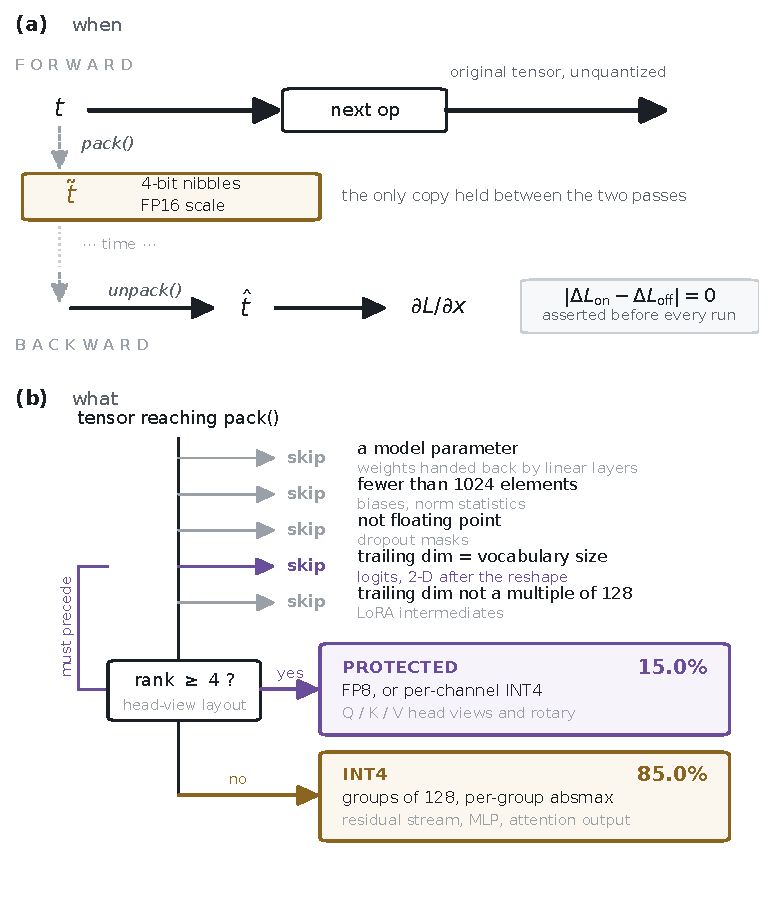
\includegraphics[width=0.7\textwidth]{fig_method.pdf}
\caption{Backward-only activation compression with rank-based dispatch.
\textbf{(a)} The forward pass uses the original tensor $t$. Only the
packed copy $\tilde{t}$ stays in memory between the two passes, and
backpropagation computes with the dequantized $\hat{t}$. So forward numerics stay unchanged. Every run asserts this before training begins: the loss
is computed with hooks disabled and enabled, and the run aborts unless the two
agree exactly. \textbf{(b)} Filters apply in the order shown. The
vocabulary-size filter must come before the rank dispatch: after the cross-entropy
reshape the logits are two-dimensional and aligned on the trailing dimension, so if a rank rule ran first, it would route them into four-bit quantization by mistake. The two
percentages are shares of stored activation elements at Llama-3.2-3B, measured
from pack-time counters over a full training run; at Llama-3.1-70B the
four-dimensional share is $11.1\%$.}
\label{fig:method}
\end{figure}

\subsection{Backward-only interception and the quantizer}
\label{sec:method_hooks}
\label{sec:method_quant}

We intercept the tensors autograd retains through PyTorch's
\texttt{saved\_tensors\_hooks}, so that $\texttt{pack}: t \mapsto \tilde{t}$ and
$\texttt{unpack}: \tilde{t} \mapsto \hat{t} \approx t$. The forward computation
consumes $t$, not $\hat{t}$, and only $\tilde{t}$ stays in memory between the
passes: forward numerics are unchanged by the compression, which we verify
bit-for-bit at every configuration. The gradient is not exact, since
backpropagation computes with $\hat{t}$, and which tensors can absorb that error
is the subject of \S\ref{sec:predicate}. Prior activation-compressed training
takes the same backward-only form
\citep{chen2021actnn,liu2022gact,hyclora2025}. The alternative, a
straight-through estimator on a quantized forward activation, is
quantization-aware training and saves nothing here, because the construction
keeps the original tensor in the graph.

The quantizer is symmetric INT4 with a per-block absmax scale over $g = 128$
elements along the trailing axis, two codes per byte, giving $4 + 16/g = 4.125$
bits per element. INT4 rather than FP4 (E2M1) because \S\ref{sec:predicate}
shows the two differ only on tensors we do not store at four bits anyway.
Appendix~\ref{app:config} gives the packing layout, the padding rule and the
dequantization path.


\subsection{Protecting the head views}
\label{sec:method_qk}

Tensors of rank four are stored differently. In a decoder-only block with
FlashAttention the $O(L^2)$ attention matrix is never materialized, so the
four-dimensional tensors retained for backward are the attention head views
$(B, H, L, d_h)$ together with the rotary embedding tables. Of these, the query
and key views are the ones that cannot handle four bits. Compressing them
drops gradient cosine to $0.36$ against $0.99$ for the value views
(\S\ref{sec:predicate}). The rule we apply is the following.\footnote{The implementation tests $\mathrm{rank}(t) = 4$. Instrumenting the
dispatch on Llama-3.2-3B, all $1{,}064$ tensors that pass the filters over two
optimizer steps are of rank $2$, $3$ or $4$ with $224$, $392$ and $448$
respectively and none is of higher rank, so the two forms coincide here. We
state the rule as $\geq 4$ because the property that matters is the head-view
layout rather than the exact rank.} It over-selects: of the 224 rank-4 tensors a step retains at 3B, 112 are rotary
tables and the other 112 are head views, 56 query and 56 key or value, so rotary
is half the population by count and $5.9\%$ of it by element.

\begin{equation}
\tilde{t} =
\begin{cases}
Q_{\text{protected}}(t) & \text{if } \mathrm{rank}(t) \geq 4 \\
Q_{\text{INT4}}(t) & \text{otherwise.}
\end{cases}
\label{eq:dcr_dispatch}
\end{equation}

FP8 (E4M3) at blockwise granularity costs
$8.125$ bits per element on the affected tensors and produced no damaged run in
eight seeds. Symmetric INT4 with the scale computed along the channel axis
rather than within blocks of the head dimension stays at four bits, $4.105$ bits per element at our sequence lengths, since one scale per channel costs $16/L$ rather than the $16/g = 0.125$ of one scale per group and produced one damaged run in eight, at a mean cost of $1.7\%$ in held-out perplexity. We use FP8 by default and report per-channel as the option when an eight-bit float format is unavailable; \S\ref{sec:dose} compares them.

Rank is a stand-in for the property that actually matters. Four-dimensional tensors are not automatically sensitive (ActNN compresses convolutional feature maps to two bits \citep{chen2021actnn}). And the rule over-selects: rotary tables are
four-dimensional, are re-saved by every layer, make up $5.9\%$ of
four-dimensional elements, and are barely affected at four bits. Promoting them
wastes $0.035$ bits per element, $5.9\%$ of what the promotion costs in total.
A rule that inspected the consuming operator would avoid this. We did not implement one, and we note the gap between our rule and our implementation.

\subsection{Exclusions and filter order}
\label{sec:method_filter}

Not every tensor reaching \texttt{pack} is an activation. The following filters
apply in order, and the order matters:

\begin{enumerate}\itemsep2pt
\item \textbf{Parameters.} We record the storage pointers of all model
parameters before training and skip any tensor sharing one. Without this,
\texttt{nn.Linear} backward passes the weight matrix to \texttt{pack} alongside
its input, and quantizing it corrupts the weight gradient. GACT applies the same
guard \citep{liu2022gact}.
\item \textbf{Small tensors.} Fewer than $1024$ elements, eight groups at
$g{=}128$. The threshold is set rather than derived; we did not tune it.
\item \textbf{Non-floating-point.} Dropout masks and index tensors. At our LoRA
dropout rate these are $22.7\%$ of the elements reaching \texttt{pack} at
$L{=}4096$ and $32.2\%$ at $L{=}512$, counting distinct storage and excluding
model parameters.
\item \textbf{Vocabulary-sized tensors.} Logits of shape $(B \cdot L, |V|)$.
This filter must come before the rank dispatch: logits are two-dimensional after the
cross-entropy reshape, so a rank-based rule alone would route them into four-bit
quantization. GACT likewise assigns 32 bits to the classification head, after
observing on an image benchmark that the context tensor saved by the
cross-entropy operator is the most sensitive in the network \citep{liu2022gact}.
\item \textbf{Misaligned tensors.} Those whose trailing dimension is not a
multiple of $g$; a group would otherwise span a channel boundary. In practice
this excludes only the rank-$r$ LoRA intermediates.
\end{enumerate}

Surviving tensors are dispatched by rank as in
Equation~\ref{eq:dcr_dispatch}. Under this policy we compress tensors carrying
$68.5\%$ of the activation elements reaching \texttt{pack} at $L{=}4096$ and
$55.3\%$ at $L{=}512$, over the same denominator: distinct storage, parameters
excluded. The difference between the two lengths is that the excluded dropout
masks and logits are a larger share at short context: $32.2\%$ and $12.3\%$
against $22.7\%$ and $8.7\%$.

\medskip
\label{sec:method_dtype}
Two library behaviors store activations at float32 in a configuration that is
otherwise four-bit. \texttt{LlamaRMSNorm} upcasts its input to compute the
variance and retains that float32 intermediate for backward, at two sites per
block; \texttt{prepare\_model\_for\_kbit\_training} casts every non-\texttt{Params4bit}
parameter to float32, and PEFT's adapter forward then matches its input, at four
sites per block. Restoring both to bfloat16 saves 2.82 and 5.72\,GB
respectively at $B{=}2$, $L{=}4096$, two bytes per stored element, as the
tensor shapes predict, and costs no time. Appendix~\ref{app:config} gives the
one-at-a-time decomposition. Every configuration in this paper applies both
corrections, so they are part of the baseline rather than a result.

\medskip
\label{sec:method_safeguard}
A step whose gradient contains a non-finite value is skipped: the optimizer
state is left untouched and the scheduler is not advanced. Twenty-one of the
500 optimizer steps in a Qwen2.5-3B run trigger this. We report the guard as part of
the configuration rather than as a result. What we can say about it is limited.
Turning it off on Qwen2.5-3B, the only model whose counter is
non-zero, flags 21 steps in both directions, and the two index lists differ by
exactly the running count of skips ($\text{off}[i] - \text{on}[i] = i$ for all
21) so the same points in the data trigger either way and the guard changes
only whether such a step is applied. The unguarded run scores $42.4\%$ against
$68.2\%$ for the nearest guarded one. That pair is not a
controlled comparison: the two differ in body encoding, and the guarded
population on this model itself spans $40.0\%$ to $75.6\%$, which contains the
unguarded figure. Appendix~\ref{app:config} lists both runs and the
configuration fields on which they differ.


\section{Setup and Motivation}
\label{sec:exp}

\subsection{Setup}
\label{sec:setup}

Llama-3.2-3B-Instruct, Llama-3.1-70B-Instruct and Qwen2.5-3B-Instruct, all on a
single NVIDIA GB10 with 128\,GB of unified memory. Because host processes share
that pool we cap the training container at 120\,GB and abort above a
reserved-memory ceiling of 100\,GB (115\,GB for the $L{=}3072$ cells and for
the uncompressed slope measurement at $L{=}1024$ and 1536), and we report \texttt{max\_memory\_reserved} throughout: on a
unified-memory device it is the reserved figure, not the allocated one, that
approaches the physical limit.

Fine-tuning is GSM8K \citep{cobbe2021gsm8k}, rank-16 LoRA on the attention
projections, two epochs at 3B (3{,}736 optimizer steps) and 500 steps at 70B.
Accuracy is 8-shot chain-of-thought with greedy decoding under a fixed stop
rule; held-out perplexity is 200 WikiText-2 windows of 512 tokens.

Six arms appear throughout the 3B experiments, and Table~\ref{tab:arms} names them.
An arm is fixed by two choices: the \emph{body encoding}, applied to every
compressed tensor of rank two and three, and the storage of the
four-dimensional \emph{head views}. Under the method names of
\S\ref{sec:method}, the uncompressed arm is Standard, the two arms that leave
the head views at blockwise four bits are Four-bit, and the three that route
them to a protected encoding are DCR (Dimension-Conditional Routing). The
uncompressed arm stores no activation at reduced precision and is therefore
independent of the body encoding. The rest of the paper refers to arms by the
names in the table; the letters appear only where space is short, in
Figure~\ref{fig:dose_response} and in the appendix tables.
The number of seeds per arm varies with what each claim requires and is stated
in every table. Appendix~\ref{app:config} gives the full configuration, the
70B checkpoint, the sequence-length statistics, and the evaluation protocol.

\begin{table}[htbp]
\centering
\small
\caption{The six arms at Llama-3.2-3B. \emph{body} is the encoding applied to
tensors of rank two and three; \emph{head views} is the storage of the
four-dimensional attention head views. Appendix~\ref{app:arms} gives the
configuration triple that identifies each arm in the released records.}
\label{tab:arms}
\begin{tabular}{cllllr}
\toprule
& arm & method (\S\ref{sec:method}) & body & head views & seeds \\
\midrule
C & the uncompressed arm    & Standard & ---  & ---              & 2 \\
A & the blockwise arm       & Four-bit & E2M1 & blockwise 4-bit  & 8 \\
D & the INT4 arm            & Four-bit & INT4 & blockwise 4-bit  & 3 \\
F & the per-channel arm     & DCR      & E2M1 & per-channel INT4 & 8 \\
B & the FP8 arm             & DCR      & E2M1 & FP8 (E4M3)       & 8 \\
E & the INT4-body variant   & DCR      & INT4 & FP8 (E4M3)       & 3 \\
\bottomrule
\end{tabular}
\end{table}


\subsection{Compression is what makes 70B fit}
\label{sec:70b_memory}

\begin{table}[t]
\centering
\small
\caption{Peak reserved memory for Llama-3.1-70B LoRA fine-tuning on a single
NVIDIA GB10 (128\,GB unified memory), batch size 1, synthetic fixed-length
sequences. NF4 weights, adapters, and optimizer state occupy 39.65\,GB before
any activation is retained. Standard LoRA does not compress activations and is
independent of the body encoding.}
\label{tab:70b_memory}
\begin{tabular}{lrrrr}
\toprule
$L$ & Standard & \, + recompute & 4-bit, Q/K at FP8 & 4-bit, Q/K per-channel \\
\midrule
1024 & 71.37 & 44.53 & 63.23 & 61.64 \\
1536 & 86.13 & 45.77 & --- & --- \\
2048 & abort\dag & 48.63 & 76.85 & 74.74 \\
3072 & 130.4\ddag & \textbf{52.67} & 90.95 & 87.85 \\
\bottomrule
\end{tabular}

\vspace{2pt}
\footnotesize
\dag\ Out of memory at $L{=}2048$: the watchdog aborted on first observing
reserved memory above its 100\,GB ceiling, at 100.62\,GB against a predicted
100.90. Only 41.18\,GB was live at that instant, so the reservation reflects
allocator behavior under pressure rather than a lower bound on the working set.
\ddag\ Extrapolated from $L{=}1024$ and $L{=}1536$.
\end{table}

This is the motivation for the rest of the paper. On a
single 128\,GB device, Llama-3.1-70B LoRA fine-tuning aborts at $L{=}2048$
without compression and runs to $L{=}3072$ with it, at 90.95\,GB against an
extrapolated 130.4. NF4 weights, adapters and optimizer state take 39.65\,GB
before any activation is stored, so the activation store is what decides the budget. Gradient checkpointing reaches an even lower peak, 52.67\,GB, and
\S\ref{sec:overhead} is where the two are compared; the case for compression is
that it costs 7\% in step time at this scale where recomputation costs 43\%.

These are single runs at each length, and one run cannot separate a
configuration from its seed. That is a real limitation for a capability claim, and it is also the reason this section is short. What the paper contributes is the check that such numbers would have to pass, not the numbers themselves. Appendix~\ref{app:config} records the configuration.

Figure~\ref{fig:vram} plots the same measurements against sequence length.
The uncompressed line is fitted to its two uncensored points, and the
compressed lines by least squares over their three points; a two-point fit of
the FP8 arm through $L{=}2048$ and 3072 would place its crossing at 5763
instead of 5815. The uncompressed run at $L{=}2048$, which the watchdog
stopped at 100.62\,GB against 100.90 predicted, is right-censored and does not
constrain the slope. Weights, adapters and optimizer state are a 39.65\,GB
constant that compression does not touch, which is why the compressed curves
converge on the baseline's slope rather than on a fraction of its height.

\begin{figure}[htbp]
\centering
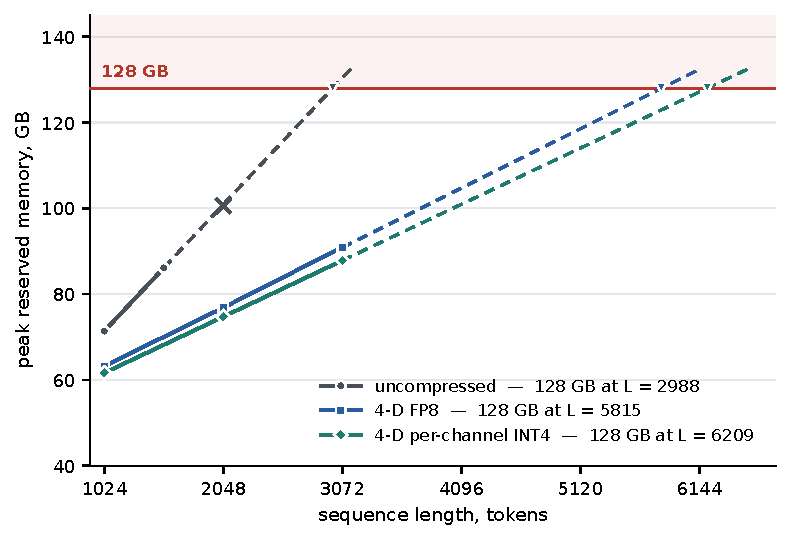
\includegraphics[width=0.808\textwidth]{fig1_vram_scaling.pdf}
\caption{Peak reserved memory against sequence length at Llama-3.1-70B. Round,
square and diamond markers are measurements; dashed segments extrapolate to the
128\,GB ceiling, where a triangle marks each crossing. The cross at $L{=}2048$
is the uncompressed run the watchdog stopped.}
\label{fig:vram}
\end{figure}


\subsection{The recomputation alternative}
\label{sec:overhead}

Recomputation reaches a lower peak than compression at every length we measured
(\S\ref{sec:70b_memory}), so what justifies compression is time rather than
memory. At Llama-3.2-3B, $B{=}2$, $L{=}4096$, recomputation reaches
$0.43\times$ the uncompressed peak at $1.31\times$ the step time while four-bit
compression with FP8 head views reaches $0.70\times$ at $1.18\times$; neither wins on both. The time gap widens with depth: at Llama-3.1-70B and $L{=}1024$,
recomputation costs 43\% against compression's 7\%, because recomputation
replays a forward pass through 80 transformer blocks rather than 28 while
quantization cost scales with stored elements. As a ratio (the only comparison available at $L{=}3072$, where the uncompressed baseline does not fit), recomputation costs $1.11\times$ compression at 3B, $1.34\times$ at 70B and $L{=}1024$, and $1.32\times$ at 70B and $L{=}3072$. Appendix~\ref{app:config}
gives the full timing tables, the two protected encodings' timings (42.76
against 42.29 seconds at 70B, not separable on one run each), and the extrapolated length at which each budget is used up.

The two can be combined: recomputation discards activations that are never stored,
compression reduces those that are, and a configuration that checkpoints some
blocks and compresses the rest is available and unexplored here. 


\section{What Determines Whether Compression Works}
\label{sec:whatmatters}

\subsection{Which tensors are sensitive, and why}
\label{sec:predicate}

Section~\ref{sec:method_qk} routes four-dimensional tensors to a protected precision without saying which of them needed protecting. This section establishes that only two do, identifies the mechanism, and shows that the identification predicts training outcomes.

\medskip
Fix a checkpoint and a batch, let $g^\star$ be the gradient with nothing
compressed and $g_{\mathcal{F}}$ the gradient with compression applied only to
the tensors a filter $\mathcal{F}$ selects, and report
$\cos(g_{\mathcal{F}}, g^\star)$ over the concatenated parameter gradients. One
role is compressed at a time and everything else passes through untouched, so any drop in the cosine comes from that role alone. Appendix~\ref{app:probe} explains how we attribute tensors to roles: storage-pointer tagging, the re-materialization that rotary embedding and \texttt{repeat\_kv} perform, and the 6--12\% of head views (7 to 13 of the 56 query views) that the tagging misses. It also gives the direction of the resulting bias, which is conservative for the claim below.


\begin{figure}[htbp]
\centering
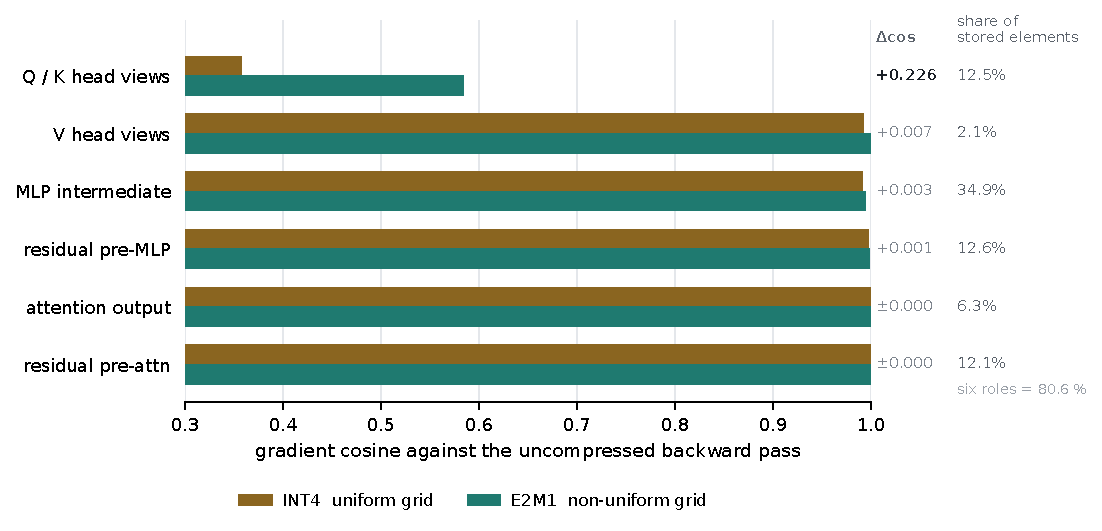
\includegraphics[width=\textwidth]{fig3_per_role.pdf}
\caption{Gradient cosine against the uncompressed backward pass, by role, under
the two four-bit grids. Each role is compressed in isolation while every other
tensor passes through uncompressed, so any drop in the cosine comes from that role alone. Shares are of the stored elements the probe attributes to a role
(Appendix~\ref{app:probe}).}
\label{fig:per_role}
\end{figure}

Figure~\ref{fig:per_role} compares uniform INT4 against non-uniform E2M1 at four bits, role by role. The two grids differ by $0.226$ in gradient cosine on the query and key head views and by less than $0.01$ everywhere else on the residual stream before and after attention, on the MLP intermediates, on the attention output, and on the value head views. Query and key account for $12.5\%$ of the elements attributed in this measurement; the MLP intermediates, at $34.9\%$, are nearly three times larger and show a difference of $0.003$.

The value head views are the informative case. They have the same rank as $Q$ and $K$, are produced by an adjacent projection of the same input, and differ only in where they enter the attention computation. Compressing them to four bits leaves gradient cosine at $0.992$; compressing $Q$ and $K$ leaves it at $0.358$.

$Q$ and $K$ enter the attention scores as $S = QK^\top/\sqrt{d_h}$, which is then exponentiated. A perturbation in either factor gets amplified twice: once by the product, and once by the softmax. The softmax normalizes over the sequence, so shifting one logit relative to its neighbors redistributes probability mass multiplicatively. $V$ is multiplied by the already-normalized weights, and the output projection comes after the attention output. In both, the perturbation passes through linearly.

\citet{actcomp2026} derive the general form. For a nonlinear operator the input-gradient error propagates as a product of Jacobians, $\Delta G_X^i = \Delta G_X^l J^{l-1} \cdots J^i$, whose Frobenius norms they measure well above 1 at depth; for linear operators the error is unbiased and does not build up. Their experiment shows the same pattern as ours, one level up (operators rather than tensors): compressing linear operators alone leaves Qwen3-4B accuracy unchanged, while compressing softmax alone drops it to $0.002$. We locate the effect in the gradients themselves and in a specific pair of tensors.

The rank-4 rule also selects the rotary tables. They are essentially unaffected at four bits ($\cos = 0.9997$, E2M1 grid, step 0), so promoting them costs 0.035 bits per element for no benefit (\S\ref{sec:method_qk}). 

\begin{table}[htbp]
\centering
\small
\caption{Gradient cosine by depth under four treatments of the query and key
head views, at step 0, before fine-tuning. Values are the mean over the LoRA $B$
parameters of each layer: at initialization $B = 0$, so the gradient with
respect to $A$ vanishes and the signal is carried entirely by $B$. The values
are from the first of the two probes described above; the arm-level cosines of
Table~\ref{tab:dose_x} come from its repeat seven minutes later.}
\label{tab:layerdepth}
\begin{tabular}{lccc}
\toprule
$Q/K$ stored as & layer 0 & layer 13 & layer 27 \\
\midrule
INT4, blockwise        & 0.435 & 0.818 & 0.815 \\
E2M1, blockwise        & 0.518 & 0.849 & 0.942 \\
INT4, per-channel      & 0.828 & 0.974 & 0.992 \\
FP8                    & 0.984 & 0.998 & 0.999 \\
\bottomrule
\end{tabular}
\end{table}

\medskip
The filters that produce this axis compress the head views and pass everything
else through, so two configurations that treat the head views alike receive the same measurement by design, no matter what else differs between them. We tested
what that blindness costs when the probe is used to predict. The FP8 arm and its INT4-body variant (Table~\ref{tab:arms}) route the head views to FP8 and differ only in
the body encoding, E2M1 against INT4. The probe therefore gives both a cosine
of 0.9919 and a norm ratio of 0.9518. Before measuring, we pre-specified the
prediction that their training endpoints would be indistinguishable in
geometry as well.

They were not. The mean cosine between the row spaces of two runs' LoRA updates
is 0.1339 in the FP8 arm and 0.1314 in the INT4-body variant, and the two
arms' pair values do not overlap. Sample size does not explain the gap: a variance-component model over the eight-run arms puts it at $z = 5.9$ to $7.1$. The metric does not explain it either: row-space angles are exactly scale-invariant, and the divergence is in the largest singular directions, not the smallest. The body encoding has no visible effect anywhere the probe and the perplexity measurements look: every body role
stays above $\cos = 0.99$ under either grid, and the INT4-body variant's mean
falls inside the FP8 arm's range on all four held-out corpora. It does have an effect at the endpoint: the INT4-body variant's adapters finish with a mean update norm of 24.5 against 31.0 for the FP8 arm, the same level as the uncompressed
runs.

We report this as a limit on what the probe can tell us. It orders configurations
by how faithfully the backward pass survives compression of the tensors it
compresses. It does not determine where training ends up, because an axis it
does not measure moved the endpoint while leaving both of its numbers, and four
corpora, unchanged.


Under blockwise four-bit compression the first transformer layer is consistently the most sensitive, its gradient cosine falling 0.31--0.42 below the deeper layers across two probes run seven minutes apart. That spread narrows to 0.15 under a per-channel scale and to 0.014 under FP8, tracking the aggregate cosine. Layer 0 is the only depth whose cosine moves noticeably between the two probes by up to 0.026, against 0.011 at layers 13 and 27, so we report its gap as a range rather than a point. We do not know why the first layer is worse. A per-layer routing rule that protects only the earliest blocks is a natural extension we did not try.

\medskip
If the two grids differ only on $Q$ and $K$, then protecting $Q$ and $K$ should make the choice of grid irrelevant. Table~\ref{tab:2x2} tests this directly by crossing the body encoding with the treatment of four-dimensional tensors.

\begin{table}[htbp]
\centering
\small
\caption{WikiText-2 perplexity crossing the body encoding with the treatment of
four-dimensional tensors. Each cell is one seed (42) at 3B.}
\label{tab:2x2}
\begin{tabular}{lrrr}
\toprule
& 4-D at four bits & 4-D at FP8 & 4-D effect \\
\midrule
INT4 body & 17.694 & 15.925 & $+1.769$ \\
E2M1 body & 15.780 & 15.933 & $-0.153$ \\
\midrule
body effect & $+1.914$ & $-0.008$ & \\
\bottomrule
\end{tabular}
\end{table}

The body encoding is worth $1.91$ perplexity points when the head views are left at four bits and $-0.008$ when they are not; the effect vanishes. Seen from the other side, upgrading the head views is worth $1.77$ points under an INT4 body and $-0.15$ under E2M1. There is no main effect, only an interaction, and it is the interaction the per-role probe predicts.

Table~\ref{tab:2x2} is one seed per cell, and seed 42 is the lowest of the eight blockwise runs on WikiText-2, so its cell values are not stable on their own. The same $2 \times 2$ on in-distribution GSM8K perplexity, with three to eight seeds per cell, has the same shape: the body encoding moves it by 0.077 when the head views are at four bits (2.6415 against 2.5645) and by 0.002 when they are at FP8 (2.5592 against 2.5577), and upgrading the head views moves it by 0.082 under an INT4 body and 0.007 under E2M1. With head views at FP8, an INT4 body reaches in-distribution perplexity 2.5592 across three seeds (sd 0.0013) against 2.5580 for the uncompressed baseline (two seeds, sd 0.0009), and a gradient norm of $0.62$ against $0.61$ for an E2M1 body and $0.59$ uncompressed, while the same INT4 body with head views at four bits reaches $2.6415$ and $586$.


\subsection{Within a tensor, magnitude does not identify what to protect}
\label{sec:anchor_ablation}

The method of \S\ref{sec:method} allocates precision \emph{between} tensors.
The within-tensor approach is the more obvious one, and it is the one we
built first. It fails.

Quantization error under a per-group absolute-maximum scale is bounded by the
group's maximum: a group whose largest element is $m$ has step size $m/7$ at
four bits, so the groups holding the largest values contribute most to the error
in absolute terms. Scoring groups by max-abs and promoting the top $K\%$ to FP8
targets the error where it is largest, at $4K/100$ bits per element. This is the
within-tensor version of outlier-aware weight quantization
\citep{dettmers2022llmint8}, and HyC-LoRA applies a related idea to buffered
activations \citep{hyclora2025}.

Max-abs ranks groups by how badly the quantizer reconstructs them. Whether a
group's error matters is a different question, and the two rankings are almost unrelated. Over 15 checkpoints of a 300-step run we ranked the 128-element
groups of each residual hidden state by their maximum absolute value and,
separately, by the norm of the gradient flowing through them. The Spearman
correlation between the two rankings is 0.13. The overlap between the top 20\%
under each is 0.248, against 0.200 expected by chance: selecting on max-abs is
barely better than selecting at random.\footnote{Llama-3.2-3B, BF16 base
weights, $B{=}1$, $L{=}512$, measured every 20 steps with three samples per
point; this predates the E2M1 body encoding and the rank-4 routing rule.}

Section~\ref{sec:predicate} explains why the two rankings disagree. The residual stream
carries activations whose dynamic range, absolute maximum over median absolute
value, is 9362 at its largest against 125 for the query views, a factor of 75
(the largest per-tensor ratio in the per-role probe of \S\ref{sec:predicate}:
step 0, before fine-tuning, $B{=}1$, $L{=}512$), and yet it is entirely insensitive to four-bit compression while the query views
are not. A statistic that measures how extreme a tensor's values are is
measuring the wrong thing.

We compared $K{=}0$ against $K{>}0$ on three model--scale combinations. No comparison favors the anchors. One of the four, the Qwen pair with an E2M1 body, reaches nominal significance (McNemar exact $p = 0.037$), in the direction against the anchors; the other three do not (Table~\ref{tab:anchor_acc}).

\begin{table}[htbp]
\centering
\small
\caption{GSM8K accuracy with anchors against without, in percentage points.
$\Delta$ is the anchored arm minus the unanchored one, so a negative value
means the anchors did not help. Every comparison is negative except the 70B
pair, whose difference is well inside its own standard error. The 3B rows use
the in-training evaluation (500 problems, 256-token budget, no stop sequences),
the 70B row the unified re-evaluation of Table~\ref{tab:accuracy} (200
problems, 512 tokens, stop sequences), and the Qwen rows a 500-problem
re-evaluation at 512 tokens without stop sequences; comparisons are made within
a row only.}
\label{tab:anchor_acc}
\begin{tabular}{llrl}
\toprule
Model & Comparison & $\Delta$ & \\
\midrule
Llama-3.2-3B & $K{=}0.2$ vs.\ $K{=}0$, paired & $-1.40$ & $t = -1.15$, $\mathrm{df} = 2$ \\
Llama-3.1-70B & $K{=}0.2$ vs.\ $K{=}0$ & $+0.50$ & $n{=}1$ each, difference SE 3.2 \\
Qwen2.5-3B & $K{=}0.2$ vs.\ $K{=}0$, INT4 body & $-2.60$ & McNemar exact $p = 0.24$ \\
 & $K{=}0.2$ vs.\ $K{=}0$, E2M1 body & $-3.80$ & McNemar exact $p = 0.037$ \\
\bottomrule
\end{tabular}
\end{table}

The 3B comparison pairs by seed and is limited to the three seeds for which both arms were evaluated under the same protocol and neither run is a duplicate training (\S\ref{sec:lottery}). The Qwen comparisons are
paired by question. All arms answer the same 500 items, so McNemar's test
applies where per-item records exist; the two INT4-body arms disagree on 103 of the 500 items with a net difference of 13, and the two E2M1-body arms on 75 with a net difference of 19. We report the direction because it is
consistent across four comparisons, and we do not claim it is established.

\medskip
They do have an effect. On Qwen2.5-3B, whose activation outliers are an order of
magnitude larger than Llama's, the number of optimizer steps skipped for
non-finite gradients falls from 21 at $K{=}0$ to zero at $K{=}0.4$: promoting
the largest groups does suppress the overflow that the safeguard of
\S\ref{sec:method_safeguard} otherwise catches. The mechanism works, but it is redundant. The safeguard already handles those steps at no cost in bits, and
the precision the anchors consume buys nothing.

\medskip
The two ways of allocating precision are not interchangeable. Within a tensor,
the largest values are the ones a max-abs scale already handles best in relative terms. Between tensors, the question is which tensors sit on a path
that amplifies error, and \S\ref{sec:predicate} shows that question has an answer.


\subsection{How much precision the head views need}
\label{sec:dose}

Section~\ref{sec:predicate} established that the query and key views are the
sensitive tensors. This section asks how sensitive: we vary the precision at
which they are stored across four settings, hold everything else fixed, and
measure held-out perplexity over eight seeds per setting.

The four settings differ only in how the head views are quantized, and are
identified by the gradient cosine each produces on a fixed checkpoint
(\S\ref{sec:predicate}):

\begin{table}[htbp]
\centering
\small
\caption{The four points of the dose--response curve. Cosines come from the
per-role probe of \S\ref{sec:predicate} and share its attribution gap: each is
measured with the query views the pointer map misses left uncompressed, which
biases all four in the same direction and toward one, so the ordering is
unaffected and the absolute values are conservative. The bits column is the
cost on the head-view tensors themselves; over the whole activation store the
per-channel arm measures 4.1205 bits per element against 4.125 for blockwise
and 4.727 for FP8.}
\label{tab:dose_x}
\begin{tabular}{llcc}
\toprule
Storage & $\cos(g, g^\star)$ & bits/elem & how it arises \\
\midrule
INT4, blockwise (D)         & 0.371 & 4.125 & INT4 body, no rank-4 rule \\
E2M1, blockwise (A)         & 0.587 & 4.125 & E2M1 body, no rank-4 rule \\
INT4, per-channel scale (F) & 0.910 & 4.105 & rank-4 rule, four-bit \\
FP8 (E4M3), blockwise (B, E) & 0.992 & 8.125 & rank-4 rule, eight-bit \\
\bottomrule
\end{tabular}
\end{table}

The first two come from letting the body encoding handle the head views; the
gradient measurement in \S\ref{sec:predicate} showed that INT4 and E2M1 differ
only on these tensors, and here that difference becomes the first two points of
a dose--response curve. The last two are the two protected encodings of
\S\ref{sec:method_qk}.


\begin{figure}[htbp]
\centering
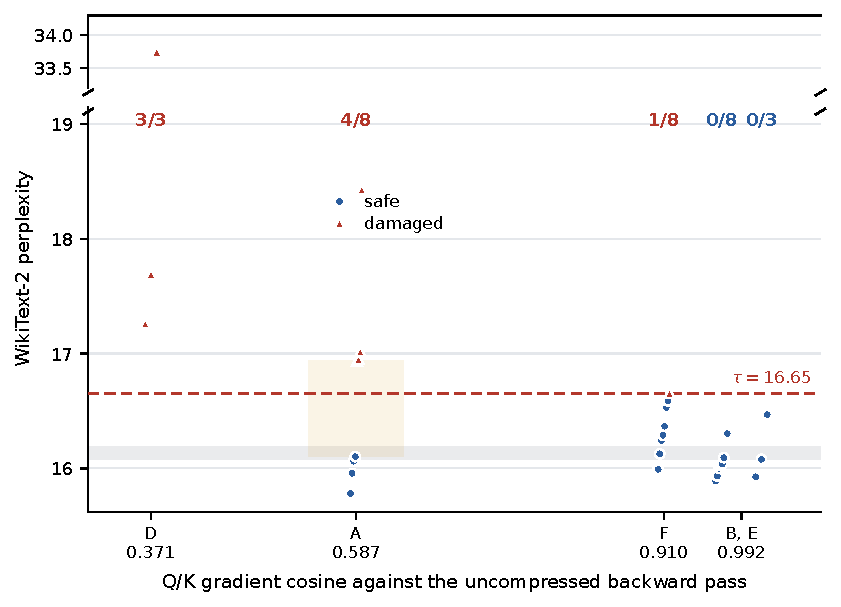
\includegraphics[width=0.859\textwidth]{fig2_dose_response.pdf}
\caption{WikiText-2 perplexity of every 3B run against the Q/K gradient cosine
of its configuration, one mark per run. The dashed red line is the
pre-specified threshold $\tau = 16.65$; the counts above each column are runs
above it. The gray band spans the uncompressed adapter (16.08) to the
un-fine-tuned base model (16.19), and the pale band at A (blockwise) is its
empty interval, 0.83 wide. The $y$ axis is broken for the outlier of D (INT4)
at 33.75. Ticks name the arms as in Table~\ref{tab:arms}. Left
to right the columns are D (INT4), A (blockwise), F (per-channel), B (FP8) and
E (INT4-body variant), as defined in Table~\ref{tab:arms}. The two columns at
0.992 share the storage and differ in body, E2M1 ($n=8$) and INT4 ($n=3$), and
are drawn apart.}
\label{fig:dose_response}
\end{figure}

Figure~\ref{fig:dose_response} plots every run. The pre-specified threshold is
$\tau = 16.65$: the uncompressed mean, 16.08, plus three standard deviations of
the FP8 arm as it was at pre-specification, 0.19 over its first three seeds,
fixed before any of the additional seeds were run. Under it the damage counts
are $3/3$, $4/8$, $1/8$, and $0/8$ as gradient cosine rises. Both spread
and mean move monotonically (Table~\ref{tab:dose_summary}).

\begin{table}[htbp]
\centering
\small
\caption{WikiText-2 perplexity by gradient cosine, aggregated over the runs of
each arm, with each arm's comparison against the FP8 arm in the three
right-hand columns. \emph{range} is the largest value minus the smallest,
\emph{damaged} counts runs above the pre-specified threshold $\tau = 16.65$,
and \emph{gap} is the largest gap between adjacent runs. The uncompressed row
is the reference the threshold was built from.}
\label{tab:dose_summary}
\setlength{\tabcolsep}{3pt}
\begin{tabular}{llrrrrrrrr}
\toprule
Storage & $\cos$ & $n$ & mean & sd & range & damaged & $\Delta$ ($t$, $p$) & ratio ($p$) & gap \\
\midrule
INT4, blockwise (D)     & 0.371 & 3 & 22.90 & 9.395 & 16.48 & 3/3 & ---                   & ---          & 16.05 \\
E2M1, blockwise (A)     & 0.587 & 8 & 16.66 & 0.876 & 2.65  & 4/8 & $+0.58$ (1.86, 0.10)  & 33.7 (0.03)  & 1.41 \\
INT4, per-channel (F)   & 0.910 & 8 & 16.35 & 0.233 & 0.67  & 1/8 & $+0.28$ (2.84, 0.015) & 2.37 (0.20)  & 0.16 \\
FP8, E4M3 (B)           & 0.992 & 8 & 16.07 & 0.151 & 0.41  & 0/8 & ---                   & 1            & 0.19 \\
\midrule
uncompressed (C) & --- & 2 & 16.08 & 0.007 & 0.01 & 0/2 & --- & --- & 0.01 \\
\bottomrule
\end{tabular}
\end{table}

\medskip
A damage count depends on where the line is drawn, and \S\ref{sec:limitations}
records how much. The trend can be tested without drawing one. Write $x_{ij}$
for the WikiText-2 perplexity of run $i$ in arm $j$ and
$z_{ij} = |x_{ij} - \mathrm{median}(\text{arm } j)|$ for its distance from its
own arm's center, the Brown--Forsythe transform, which turns a question about
dispersion into a question about location. The statistic is then the Spearman
correlation between an arm's gradient cosine and the $z$ of its runs, over every
compressed run at once.

Counting threshold crossings misses part of what separates these settings, because
the two four-bit schemes fail in opposite ways. Blockwise four-bit fails in the variance (Table~\ref{tab:dose_summary}). Its
mean differs from the FP8 arm at $p = 0.10$, its variance is 33.7 times larger
at $p = 0.03$, and the median-centered Brown--Forsythe statistic agrees,
$W = 9.6$ at permutation $p = 0.019$.

We use Welch's $t$ for the means and a permutation test for the variance
ratio. In Table~\ref{tab:dose_summary}, $\Delta$ is each arm's mean difference
from the FP8 arm with Welch's $t$ and its $p$, and \emph{ratio} is its variance
ratio against the FP8 arm with the exact two-sided permutation $p$ on
$|\log F|$ over all relabelings of the two arms; the $n{=}3$ and $n{=}2$ rows
are left blank on both tests. The $F$-test's normality assumption fails at
$n = 8$: 59\% of this arm's variance is carried by one run, and that is exactly the tail the $F$-test takes its $p$-value from. Appendix~\ref{app:stats} says why swapping the two tests in the other direction does not work either. The conclusion does not depend on the
choice: a permutation test of the mean difference gives $p = 0.065$.

The arm also separates into two groups. Four runs fall between 15.78 and 16.10
and four between 16.94 and 18.43, with no run in the 0.83 between them, which
is 4.4 times the standard deviation of the FP8 arm at pre-specification, the quantity
that defined the threshold. We report this as an observation rather than as a
test: with eight points, no test for two groups reaches significance unless it fixes the split position in advance (Appendix~\ref{app:stats}). None of the claims in this paper rests
on the separation. The variance ratio, the Brown--Forsythe statistic and the
dose response are all computed on the arm as a whole.

Per-channel four-bit fails in the mean, and only slightly. Its variance ratio
against FP8 is 2.37 at $p = 0.20$ and its distribution does not split into two groups
(Table~\ref{tab:dose_summary}). But it sits $1.7\%$ higher on average, at
$p = 0.015$. Its single threshold crossing is a run at
$+3.6\%$, below the lowest blockwise failure at $+5.3\%$; the threshold was
built to fall inside a gap and here there is no gap for it to fall into, so it
cuts off the top of a continuous spread instead.

\begin{table}[htbp]
\centering
\small
\caption{Dispersion against the dose axis, over every compressed run at once.
Each run's $z$ is its distance from its own arm's median; the statistic is the
Spearman correlation between the arm's score and $z$. The null reassigns runs
to arms of the observed sizes and recomputes every median before recomputing
$z$; one-sided, $10^6$ draws. Preserving the group sizes matters in the
three-arm subset, where the $n{=}3$ arm's median is one of its own points and
so contributes an exact zero to $z$.}
\label{tab:dose_trend}
\begin{tabular}{llrr}
\toprule
dose axis & runs & $\rho$ & $p$ \\
\midrule
gradient cosine  & 30, five arms                    & $-0.624$ & $3.9\times10^{-5}$ \\
gradient cosine  & 27, INT4-body variant dropped    & $-0.637$ & $1.8\times10^{-5}$ \\
gradient cosine  & 19, bits held at 4.105 to 4.125  & $-0.570$ & $5.5\times10^{-5}$ \\
bits per element & 30, five arms                    & $-0.234$ & $0.19$ \\
bits per element & 19, bits held at 4.105 to 4.125  & $+0.701$ & $1.000$ \\
\bottomrule
\end{tabular}
\end{table}

Dispersion falls as gradient fidelity rises, with no threshold anywhere in the
calculation (Table~\ref{tab:dose_trend}).\footnote{Shuffling the $z$ values
instead of reassigning runs carries the original grouping inside the statistic
and is conservative by a factor of 3.2: on the same 30 runs and the same draws
it gives $p = 1.25\times10^{-4}$.} The bits axis cannot order these arms: the
two most damaged, INT4 and E2M1 blockwise, are tied at 4.125 bits, and
per-channel INT4, which is nearly as clean as FP8, is \emph{below} both at
4.105. What predicts the damage is not how much is stored but how faithfully
the gradient survives it.


The threshold was fixed from the first three FP8 runs; recomputed from the
final eight it is 16.53 (Appendix~\ref{app:stats}). The blockwise count is
unchanged, because both values fall inside its empty band, and the per-channel
count moves from one to three. Across $2\sigma$, $3\sigma$ and $4\sigma$
definitions the blockwise arm flags the same four runs, while the per-channel
arm gives three, one and zero. Threshold sensitivity tracks the presence of a
gap: where the arm has one, the count is robust to where the line is drawn;
where it does not, the count depends only on where the line is drawn. This is why we report
the pre-specified count and the distribution together.

Compared with prior work, our threshold is strict, not loose. Our threshold sits
$3.6\%$ above the uncompressed baseline. \citet{hyclora2025} report a $5.6\%$
increase in WikiText-2 perplexity at the two-bit setting their abstract recommends, and $1.1\%$ at four bits, both as successes. The failure we describe
therefore lies inside the band that prior work reports as working, which is the
same point \S\ref{sec:related_measure} makes about the metrics: the threshold is not loose; it measures something the accepted thresholds do not.

Two settings share the FP8 point on the curve: an E2M1 body ($n{=}8$) and an
INT4 body ($n{=}3$). They agree on all four corpora, on in-distribution
perplexity, and on gradient norm (\S\ref{sec:predicate}), and neither produces a
damaged run. Once the head views are protected, the grid used for the remaining
$85\%$ of stored elements does not matter. This is why we report INT4 as the
body encoding in \S\ref{sec:method_quant}: it is the simpler grid, needing only rounding where E2M1 needs a lookup table, and at this point on the curve the two are
indistinguishable.\footnote{We make no step-time claim between them: the same
configuration measured twice on the same day differs by a factor of 1.47 in
seconds per step, so no difference between the two encodings could be seen through that noise.}


Therefore, FP8 is the safe choice: no damaged run in eight seeds, no mean
penalty, and a spread of 0.41 across eight runs against 0.01 for two
uncompressed runs. It costs
$0.60$ bits per element overall at 3B, where the head views are 15\% of the
store ($0.44$ at 70B, where they are 11\%), and requires an eight-bit floating
format.
Per-channel scaling stays at four bits and needs only nibble packing and no
FP8 support, at a mean cost of $1.7\%$ held-out perplexity and one boundary
crossing in eight seeds. Blockwise four-bit is not a usable option at either cost. It introduces run-to-run failures, and \S\ref{sec:detection} shows that no measurement taken during or after training on the task distribution detects them. Every rate in this section is for 3{,}736 optimizer steps. At 500 steps no arm is stable on held-out text, the uncompressed arm included (Appendix~\ref{app:prereg}), so the FP8 result is a statement about this training length rather than a general one.

\subsection{The failure is a property of the run, not the seed}
\label{sec:lottery}

Section~\ref{sec:dose} reported that four of eight runs under blockwise four-bit
compression exceed the damage threshold. This section characterizes those
failures: which runs fail is not determined by the seed, the degradation is a
change in variance rather than in mean, and it does not look the same on every corpus.

\medskip
We re-ran two damaged configurations from scratch under identical settings, the
same seed, the same data order, the same code, and both became safe. The
divergence is visible in the loss trace: the first two optimizer steps agree
bit-for-bit and the third does not (Table~\ref{tab:rerun}).

\begin{table}[htbp]
\centering
\small
\caption{Re-running two damaged configurations with nothing changed. Upper:
WikiText-2 perplexity of the original run against the re-run; both cross back
below the damage threshold $\tau = 16.65$. Lower: the training loss at seed
123, which agrees to six decimal places for two optimizer steps and separates
at the third.}
\label{tab:rerun}
\begin{tabular}{lrrl}
\toprule
seed & original & re-run & \\
\midrule
123  & 18.432 & 16.271 & damaged $\rightarrow$ safe \\
4042 & 16.935 & 16.351 & damaged $\rightarrow$ safe \\
\bottomrule
\end{tabular}

\vspace{0.8\baselineskip}

\begin{tabular}{lccc}
\toprule
seed 123 & step 1 & step 2 & step 3 \\
\midrule
original & 1.295640 & 1.641697 & 1.472919 \\
re-run   & 1.295640 & 1.641697 & 1.473335 \\
\bottomrule
\end{tabular}
\end{table}

These three pairs are also the only comparison with the seed held fixed for the
endpoint geometry of \S\ref{sec:dose}, where they separate the two arms.

We attribute this to non-deterministic reduction order in CUDA kernels. The same
pattern appeared on its own in a third case: an FP8 run at seed 789 was
accidentally trained twice and diverged at the same point. Both of those runs
were safe, and the FP8 arm
shows no such spread (15.999 and 16.093 on WikiText-2 for the duplicate pair).

The consequence is that a user cannot avoid this failure by choosing a
seed. Two runs of the same configuration are two random samples.

The re-runs are excluded from the damage rate. They were selected because their
originals were damaged, so counting their outcomes would bias the rate toward
whatever the re-runs happened to produce, which here would be downward, since
both came back safe. The rate of four in eight is over the original eight runs only, and the
re-runs are evidence about what a repeat draw does, not additional samples of
the rate.

The pattern is not limited to Llama or to perplexity. Two Qwen2.5-3B runs whose
recorded configurations differ only in output directory, executed at the same
commit on the same day, skipped 20 optimizer steps for non-finite gradients and
zero respectively, and scored $40.0\%$ and $70.8\%$ on GSM8K. We did not plan
that comparison and cannot compute a rate from two runs, but it is the same
phenomenon in a second model and a second measurement
(\S\ref{sec:method_safeguard}).

\medskip
If damage were seed-determined, pairing the four-bit and FP8 runs by seed would
cancel the seed effect and shrink the standard error. It does not: the paired
$t$ is 1.85 against an unpaired Welch $t$ of 1.86. Pairing recovers nothing, as expected when the pairing variable does not determine the outcome. This matches the re-run result above, where the same seed produced a safe model twice out of two.

Because the draws are independent, the eight runs are an i.i.d.\ sample and the binomial test is exact: four of eight, against zero of eight under FP8
(one-tailed Fisher exact $p = 0.038$; the direction was fixed in advance by
defining the threshold from the FP8 arm; on the 24 runs evaluated after the
threshold was fixed the count is 2 of 5 against 0 of 5, one-sided $p = 0.22$).

\medskip
Across three held-out corpora, blockwise four-bit compression does not shift the mean but does
inflate the variance:

\begin{table}[htbp]
\centering
\small
\caption{Mean difference and variance ratio between the blockwise arm and the FP8 arm, eight runs each, on three held-out corpora. Appendix~\ref{app:stats}
gives the run-selection rules behind the table.}
\label{tab:threecorpora}
\begin{tabular}{lrrrr}
\toprule
& \multicolumn{2}{c}{mean difference} & \multicolumn{2}{c}{variance ratio} \\
corpus & $\Delta$ & $t$ ($p$) & $F$ & $p$ \\
\midrule
WikiText-2   & $+0.585$ & 1.86 (0.10) & 33.7 & 0.030 \\
GovReport    & $+0.103$ & 1.31 (0.23) & 14.0 & 0.029 \\
NarrativeQA  & $+0.363$ & 0.88 (0.40) &  4.7 & 0.209 \\
\bottomrule
\end{tabular}
\end{table}

Table~\ref{tab:threecorpora} gives the result. Mean differences are Welch $t$
and variance ratios are exact permutation, for the reasons given above. No mean difference reaches $p = 0.05$. Two of the
three variance ratios do: WikiText-2 at $0.030$ and GovReport at $0.029$, with
NarrativeQA at $0.209$. The median-centered Brown--Forsythe test agrees on the
same two, at $0.019$ and $0.014$ against $0.229$ for NarrativeQA.

Reading the Brown--Forsythe statistics themselves would suggest otherwise,
since they are $9.6$, $2.9$ and $1.8$. But a statistic is only large relative
to the distribution it came from. Against its own permutation distribution each of the
first two sits in the upper tail: $9.6$ against a 95th percentile of $8.2$ on
WikiText-2, and $2.9$ against $2.3$ on GovReport. NarrativeQA's distribution is
far wider, with a 95th percentile of $10.2$, so $1.8$ there is nothing special.
The three raw statistics are on three different scales, so comparing them directly, as a shared parametric reference would invite, is not meaningful. The two additional corpora
were not pre-specified, so we read them as supporting rather than as
independent tests.

The dispersion is not measurement noise. Re-evaluating a saved adapter
reproduces perplexity to four decimal places: we checked three adapters,
including the most extreme, and the difference was $\pm 0.0000$. The two
uncompressed runs differ by 0.009. The 0.88 standard deviation under blockwise four-bit compression is variation between models, not between measurements of the same model.

\medskip
Perplexity and benchmark accuracy both measure the model through a data distribution.
The LoRA update is the model, so we compared the endpoints directly. Write
$\Delta W = (\alpha/r) BA$ for the update at one of the 112 adapter sites. We
compare the product, since the factors are identified only up to an invertible
$G$ acting as $(GA, BG^{-1})$. Two runs can then differ in how far apart their updates are, and in the subspaces those updates occupy.

They do not differ in distance. The mean Frobenius distance between two
blockwise updates is 38.8 against 37.1 for FP8, a gap of 4.6\% at exact
permutation $p = 0.25$. They differ in direction. Averaging over the sixteen
principal angles between the row spaces of $\Delta W$ at each site, two
blockwise runs sit at a mean cosine of $0.1121$ and two FP8 runs at $0.1339$:
the blockwise arm occupies more varied subspaces. Extending the measurement
to the INT4 and per-channel arms orders all four by gradient cosine without
exception, with the uncompressed pair above them all.

\begin{table}[htbp]
\centering
\small
\caption{Mean cosine of the principal angles between the row spaces of the LoRA
updates, over all within-arm pairs and all 112 adapter sites. Lower means the
two runs occupy more varied subspaces. \emph{range} is the smallest and
largest pair value in the arm; no two arms overlap. The uncompressed row is a reference point from a single pair, not an estimate.}
\label{tab:subspace}
\begin{tabular}{lrrrr}
\toprule
arm & $\cos(g,g^\star)$ & pairs & mean & range \\
\midrule
INT4, blockwise (D)  & 0.371 &  3 & 0.0829 & 0.0823--0.0840 \\
E2M1, blockwise (A)  & 0.587 & 28 & 0.1121 & 0.1113--0.1134 \\
INT4, per-channel (F) & 0.910 & 28 & 0.1231 & 0.1218--0.1242 \\
FP8 (B)              & 0.992 & 28 & 0.1339 & 0.1330--0.1350 \\
\midrule
uncompressed (C, $n{=}1$ pair) & --- & 1 & 0.1391 & --- \\
\bottomrule
\end{tabular}
\end{table}

The ninety-one within-arm pairs, the eighty-eight of Table~\ref{tab:subspace}
and the three of the INT4-body variant, do not overlap between arms at all. Under the
null that reassigns the 27 compressed runs to arms of the observed sizes, no
reassignment in $10^5$ separated four arms this way, and correlating each pair's
value with its arm's gradient cosine gives $\rho = 0.949$ at $p = 10^{-5}$;
scoring by bits per element instead gives $0.447$ at $p = 0.047$. We do not
quote a rank correlation on the four arm means, which is $+1.000$ but reaches
that value in about one reassignment in six and so carries almost no
information at four groups.

Three reference points show what these numbers mean. Two unrelated
16-dimensional subspaces of $\mathbb{R}^{3072}$ meet at a mean cosine of
$0.061$; two runs sharing a seed but differing in compression sit at $0.82$,
since LoRA's $A$ is initialized from the seed; and the within-arm values above
lie between. Reading the arms as a fraction of the interval from chance to the
uncompressed pair, INT4 recovers 28\% of it, E2M1 blockwise 65\%, per-channel
80\% and FP8 93\%. Every arm sits well above chance, and the uncompressed pair
itself sits only $0.078$ above it, so the scatter is not something compression
creates. Training pulls the endpoints toward a common direction from the start,
and compression weakens that pull by a measurable fraction.

\medskip
The three re-run pairs of \S\ref{sec:lottery} are the only place in this work
where a run is repeated with the seed held fixed, and the same measurement
applies to them. The two blockwise re-runs sit at $0.832$ and $0.829$, the same
distance apart as two runs that differ in compression scheme entirely, while
the FP8 re-run sits at $0.954$. Re-running the blockwise configuration moves the
endpoint about as far as changing the configuration does; re-running FP8 does
not. With only two pairs against one, we describe this but do not test it. Controlling the seed also makes the Frobenius distance separate the arms, where between arms it was null: the two blockwise re-runs sit at 28.4 and 32.9 against 21.5 for FP8, a ratio near 1.4, while the between-arm figure was 1.05. At the arm level, the seed variance hid the effect; the effect was there.

What the same-seed pairs do \emph{not} show is where the damage went. The two
blockwise pairs differ by a factor of 3.7 in how far their perplexities moved
apart, 2.161 against 0.584, and by 0.003 in subspace cosine. Holding the seed
fixed makes the amplification visible; it does not make the location of the
damage visible.

\begin{table}[htbp]
\centering
\small
\caption{Every dispersion measurement in this paper, tested at two levels.
\emph{Between arms} asks whether the blockwise arm is more dispersed than the
FP8 arm; \emph{within the arm} asks whether the measurement identifies which
run inside the blockwise arm is the damaged one. The parentheses on the accuracy and item-level rows repeat the within-arm test on MMLU's 14{,}042 items; the between-arm tests cannot be repeated there, because only the blockwise arm was evaluated on MMLU (\S\ref{sec:accuracy}).}
\label{tab:levels}
\begin{tabular}{lll}
\toprule
measurement & between arms & within the arm \\
\midrule
held-out perplexity      & $p = 0.03$                       & by construction\dag \\
item-level behavior     & $p = 0.001$                      & $p = 0.21$ (MMLU $0.67$) \\
LoRA subspace direction  & $p = 0.0002$, no overlap in 91 pairs & $p = 0.025$\ddag \\
LoRA update distance     & $p = 0.25$                       & $p = 0.22$ \\
benchmark accuracy       & $p = 0.31$                       & $p = 0.93$ (MMLU $0.35$) \\
\bottomrule
\end{tabular}

\vspace{2pt}
\footnotesize
\dag\ The damage label is defined by a threshold on held-out perplexity, so
perplexity separates damaged from safe runs by definition and not as a finding.
It is listed to make the circularity explicit.\\
\ddag\ Leave-one-out over the eight blockwise runs: $p$ stays below 0.05 in
three of the eight drops (0.004, 0.027, 0.041) and lies between 0.10 and 0.21 in
the other five.
\end{table}

Table~\ref{tab:levels} collects the two levels. Between arms, each test is a
two-sided permutation over the 12{,}870 relabelings of the sixteen runs, using
the variance ratio for the two run-level quantities (perplexity, and accuracy
averaged over the four benchmarks) and the difference in mean within-arm pair
value for the three pairwise ones (item disagreement, subspace cosine,
Frobenius distance). Within the arm, each test is an exact two-sided Mantel
test over the 40{,}320 relabelings of the eight runs, correlating each pair's
value with the pair's absolute difference in held-out perplexity (for accuracy,
the pair's value is the absolute difference in mean accuracy). The first column is full of significant results; the second holds one signal that is significant on paper (subspace,
$p = 0.025$) that does not survive leave-one-out (3 of 8). So no metric aligns
with damage at the run level, and this is the paper's result, not a gap in it.

Compression widens the spread of where training ends up, in weight space, in
held-out perplexity, and in item-level behavior, at the level of the
configuration. The three do not agree run by run: the one run-level signal,
in subspace direction, is nominally significant and does not survive
leave-one-out. That is what ``each run reaches a different minimum'' means in practice, and it is why no single downstream measurement detects the effect: a run that landed somewhere else is worse on some distributions and better on others, and which distributions those are changes from run to run.

For example, seed 42 of the blockwise arm scores 15.78
on WikiText-2, better than both uncompressed baselines (16.07, 16.08) and better
than the base model before fine-tuning (16.19).\footnote{The base figure comes
from an evaluation-path diagnostic run, not from the adapter sweep, since there
is no adapter to name: the un-fine-tuned model was scored on the same 200
WikiText-2 windows of 512 tokens under the same dtype policy, in a process that
also reproduced three adapter perplexities to four decimal places.} Seed 123
scores 18.43.
Compression noise perturbs the training trajectory; it does not bias it.

\medskip
The four runs flagged on WikiText-2 are not the four runs flagged elsewhere.
The threshold formula is the uncompressed mean plus three standard deviations of
the FP8 arm, taken over all eight FP8 runs since nothing was fixed in advance
there; with the three-seed standard deviation of the pre-specified rule it gives
$3/8$ and $2/8$. Applied after the fact to the other two corpora it gives
$2/8$ on NarrativeQA and $1/8$ on GovReport, and the sets overlap in one seed
each. Rank agreement between corpora is near zero for the most distant pair
(WikiText-2 against NarrativeQA, Kendall $\tau = -0.07$, $p = 0.91$).

We do not count these crossings toward the damage rate; three corpora with
independently applied thresholds would inflate it, and only WikiText-2 was
pre-specified. What they show is that the perturbation does not push every run
in the same direction. This is consistent with the explanation above. If the compression noise moves the trajectory to a different minimum rather than degrading it along a fixed axis, then the domain where that minimum is worse can change from run to run.



\subsection{In-distribution accuracy does not separate the arms}
\label{sec:accuracy}

\begin{table}[t]
\centering
\small
\caption{GSM8K accuracy, 8-shot chain-of-thought, greedy decoding with stop
sequences and a 512-token budget. 70B evaluates 200 test examples per run and
3B evaluates 200; the binomial standard error is 3.5 points and the standard
error of a difference between two configurations is 5.0.}
\label{tab:accuracy}
\begin{tabular}{llrrl}
\toprule
Model & Configuration & $n$ & Accuracy & \\
\midrule
\multirow{4}{*}{Llama-3.1-70B}
 & base model, no adapter & 1 & 91.5 & \\
 & uncompressed           & 1 & 89.0 & \\
 & FP8 head views & 1 & 88.0 & \\
 & \quad + max-abs anchors & 1 & 88.5 & \\
\midrule
\multirow{4}{*}{Llama-3.2-3B}
  & uncompressed (C)   & 2 & 52.8 & $\pm$0.4 \\
 & blockwise (A)      & 8 & 53.9 & $\pm$2.2 \\
 & FP8 (B)            & 3 & 55.7 & $\pm$2.8 \\
 & INT4 (D)           & 3 & 48.3 & $\pm$2.8 \\
\bottomrule
\end{tabular}
\end{table}

At 70B no compressed configuration differs from the uncompressed baseline by
more than one point, against a difference standard error of 5.0. At 3B the
ordering is not interpretable: the uncompressed baseline scores below two of the
three compressed configurations, and the range across seeds within a single
configuration reaches 5.5 points. Only the INT4-body configuration, which
\S\ref{sec:dose} shows corrupts gradients by two orders of magnitude, separates
at all, and even there the ranges overlap at 51.0.

We report these numbers because prior work reports them, and because they
support the claim that compression is not obviously harmful. They do not
support finer distinctions, and \S\ref{sec:detection} shows that the
distinctions that matter are invisible here.

\medskip
Our first evaluation used a 256-token generation budget with no stop sequences,
under which 98--100\% of generations reached the limit. Re-evaluating the same
adapters with stop sequences and a 512-token budget reduced truncation to
0--2\% at 70B and revealed the actual chain-of-thought length: 57 tokens for the
base model and 67--72 after fine-tuning. Accuracy moved by at most 1.5 points,
but the re-evaluation \emph{reversed} the ordering of the uncompressed and
anchor configurations at 70B ($88.0/88.5 \rightarrow 89.0/88.5$). We take that
reversal as direct evidence that sub-point differences at these sample sizes
carry no information, and report the stop-sequence numbers throughout.

At 3B the picture is different in a useful way. Re-evaluating five
adapters under the same change altered the number of correct answers by exactly
zero, although mean generation length varied from 102 to 364 tokens across them
and truncation from 20 to 136 of 200. The generations changed; the extracted
answers did not, because the answer string appears within the shorter budget in
153--188 of 200 cases (counted as generations whose answer is extracted from an
explicit ``The answer is'' statement, the \texttt{answer\_is} source in the
evaluation records). Accuracy is insensitive to the evaluation protocol as
well as to the damage.

\medskip
Held-out GSM8K perplexity agrees as well: the four 70B runs we evaluated (two blockwise, one FP8, one uncompressed) are within 0.7\%, and at 3B the eight blockwise runs span 0.004
(\S\ref{sec:detection}). The distinction appears only out of distribution
(\S\ref{sec:dose}).

\medskip
MMLU was fixed as the primary benchmark before it was run, all 14{,}042 items
at 5-shot, together with two tests: the Spearman correlation between held-out
perplexity and MMLU accuracy over the eight blockwise runs, and the mean
difference between the four runs above the damage threshold and the four below. Both are null. The correlation is $\rho = +0.31$ at exact two-sided
$p = 0.46$ over all $40{,}320$ relabelings, with the sign opposite to the
prediction; the damaged runs score $0.32$ points \emph{above} the safe ones at
$p = 0.26$ over the 70 splits.

The same pre-specification also included a positive control: whether the INT4 arm, which is damaged on every other measurement, separates from the uncompressed pair. We noted there that without this control, a null inside the blockwise arm would be uninterpretable. That control was never completed. The MMLU chain evaluated the base model, the eight blockwise runs and two of the three INT4 runs, then stopped; the FP8 arm, the uncompressed arm and the third INT4 run have no MMLU records (Appendix~\ref{app:prereg}). The two INT4 runs that were evaluated score $55.10\%$ and $56.98\%$ against a blockwise mean of $57.02\%$, but with no uncompressed cell the comparison has no reference. What shows that the measurement can detect a shift is instead a comparison that was not pre-specified: fine-tuning on GSM8K costs $2.56$ points of MMLU on the blockwise arm (the base model scores $59.59\%$ against a mean of $57.02\%$ over the eight runs), and all eight runs fall below the base model (sign test $p = 0.0078$), so the measurement sees a shift of that size without difficulty. We report this as a substitute, not as the control we had planned. Because the FP8 arm was not evaluated on MMLU, this benchmark says nothing about compression's effect on accuracy between arms; that comparison rests on the four benchmarks of Table~\ref{tab:accuracy} and \S\ref{sec:items}.

\subsection{Aggregate accuracy hides an item-level divergence}
\label{sec:items}

Section~\ref{sec:accuracy} showed that accuracy does not separate the arms.
This section looks at the same answer sheets item by item.

Accuracy on these benchmarks is one bit per item, taken from a ranking of four
choices, and the ranking is what the arms actually differ on. Because every
adapter answers the same items in the same order, two runs can be compared item
by item. Two runs from the blockwise arm disagree on $7.39\%$ of the $6{,}653$
items and two FP8 runs on $6.59\%$, a ratio of $1.12$ at exact permutation
$p = 0.001$ over all $12{,}870$ relabelings of the sixteen runs. The direction
is the same on all four benchmarks, the result is unchanged under
length-normalized scoring ($p = 0.0002$), and the worst of the 64 balanced leave-one-out splits, dropping one run from each arm, gives $p = 0.017$.

Two reference points fix the scale. The two uncompressed runs already disagree on
$6.48\%$ of items, so most of the churn (the share of items two runs answer differently) is the seed and not the compression;
compression adds $0.91$ points to that reference, of which $0.80$ is what the FP8
rule removes. Fine-tuning itself moves behavior by $13.24$ points
against the base model, so compression's whole contribution is $6.9\%$ of what
the fine-tuning does. That is an analogous ratio to the one the accuracy comparison gave, on a different axis.

\begin{table}[htbp]
\centering
\small
\caption{Item-level disagreement between two runs of the same arm, on two item sets: the four benchmarks (6{,}653 items) and MMLU (14{,}042), where only the blockwise arm was evaluated. \emph{churn} is the fraction of items answered differently; \emph{gap} is the mean absolute difference in accuracy over the same pairs.}
\label{tab:churn}
\begin{tabular}{lrrrr}
\toprule
arm & $\cos(g,g^\star)$ & pairs & churn (pp) & gap (pp) \\
\midrule
\multicolumn{5}{l}{\emph{four benchmarks, 6{,}653 items}} \\
uncompressed (C)    & ---    &  1 & 6.478 & 0.331 \\
FP8 (B)             & 0.992  & 28 & 6.594 & 0.427 \\
E2M1, blockwise (A) & 0.587  & 28 & 7.387 & 0.556 \\
INT4, blockwise (D) & 0.371  &  3 & 9.079 & 0.962 \\
\midrule
\multicolumn{5}{l}{\emph{MMLU, 14{,}042 items}} \\
E2M1, blockwise (A) & 0.587  & 28 & 15.713 & 0.464 \\
\bottomrule
\end{tabular}
\end{table}

In Table~\ref{tab:churn} the uncompressed rows are one pair and the INT4 rows
are three, so neither is an estimate; the two eight-run arms are the comparison
that is tested, and the pooled block is reported for comparison rather than as separate evidence. The two columns do not move together. Churn grows by a factor of $1.40$ from
the uncompressed pair to the INT4 arm while the accuracy gap grows by $2.91$,
so on these four benchmarks the ratio between them falls monotonically along
the gradient-cosine axis: $19.6$, $15.4$, $13.3$, $9.4$. A worse configuration does not just disagree more; fewer of its disagreements cancel out. Aggregate accuracy is not blind, only low-resolution: two runs differing on $7.4\%$ of items end up
$0.56$ points apart, because roughly as many items move one way as the other.

Within the blockwise arm, held-out perplexity still does not say which run is
which. Splitting its eight runs at the median perplexity gives a churn difference of $0.01$ points at $p = 0.91$. The dispersion is a property of the
configuration, and it does not turn into a per-run label on this axis any
more than it did on the others.

On MMLU only the blockwise arm was evaluated (\S\ref{sec:accuracy}), so the between-arm test cannot be repeated there. Two blockwise runs disagree on $15.71\%$ of MMLU items (28 pairs, 14.65 to 17.05\%), more than on the four benchmarks, while their accuracies stay within $0.46$ points of each other on average (Table~\ref{tab:churn}). Within the blockwise arm, the split at the median perplexity gives a churn difference of $+0.01$ points at $p = 1.00$: held-out perplexity does not say which run is which on either item set.


\subsection{What the training run does not tell us}
\label{sec:detection}

\begin{figure}[htbp]
\centering
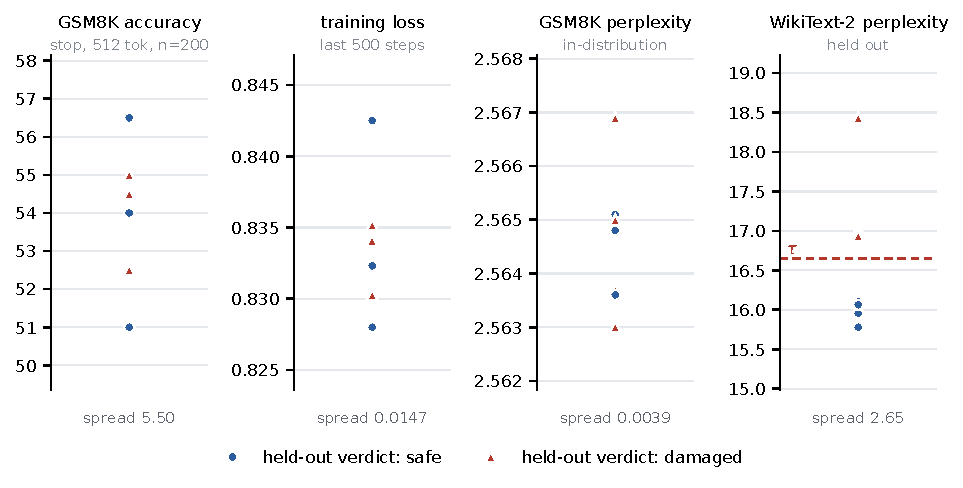
\includegraphics[width=0.984\textwidth]{fig4_insensitivity.pdf}
\caption{The same eight blockwise runs at 3B under four measurements. Color
marks the pre-specified verdict, which is defined on held-out perplexity.
Only that panel separates the colors: task accuracy, training loss and
in-distribution perplexity interleave the two groups completely. Accuracy is
the unified protocol of \S\ref{sec:setup}; training loss is the mean over the
final 500 optimizer steps. The figure under each panel is the spread across the
eight runs, in that panel's units.}
\label{fig:insensitivity}
\end{figure}

The previous section compared arms. This one asks the harder question inside a
single arm: given the eight blockwise runs, four of which the threshold calls
damaged, does anything observable during training say which four? Every
measurement we could make was blind to it (Figure~\ref{fig:insensitivity}), and that matters for how methods of this kind are evaluated, since prior work reports task accuracy and task accuracy is the least sensitive quantity we measured.

Damaged runs average 53.25\% against 54.50\% for safe ones: the right direction, but not separable (exact two-sided permutation $p = 0.51$). Training loss, averaged over the final $500$ optimizer steps, spans $0.828$ to $0.843$ across the eight blockwise runs; the damaged four average $0.836$ against $0.834$ for the safe four, a difference of $0.001$ with exact two-sided permutation $p = 0.71$. No threshold on training loss separates them, and the ordering by loss does not even go in a consistent direction. The contrast is in scale: loss spans $0.015$ across runs whose held-out perplexity spans $2.65$.

That comparison still mixes in the data order, since those eight runs differ by
seed. The re-run pairs of \S\ref{sec:lottery} remove even that. Seed 123 ends
2.16 perplexity above its re-run on WikiText-2, and nothing in the two loss
traces ever showed it. Over 3{,}736 steps the windowed RMS of their loss
difference stays between $0.005$ and $0.010$ while the step-to-step variation
within either run is $0.13$ to $0.18$: the separation never reaches a tenth of
the noise of the batch the two runs share. It does not build up over time either. Across all three re-run pairs it grows by a factor of only 1.4 to 1.7 between the first hundred steps and the last, so whatever produces the endpoint gap does not show up in the loss as something that accumulates. The blockwise pairs sit about 2.3 times higher
than the FP8 pair from the first window onward, but with two pairs against one
we do not test this. The claim is about the loss and not about the models: a single number can stay flat while the parameters move apart, and we did not
measure the weight-space trajectory.

Pre-clipping gradient norms are strongly format-dependent (Table~\ref{tab:graddetect}): INT4 bodies average 586 with every step clipped, the blockwise arm averages 1.21 with 75\% clipped, and the FP8 arm averages 0.61 with 0.4\% clipped, matching the single uncompressed run for which we have a gradient trace (0.59; we added this logging after our other uncompressed runs). Within the blockwise arm, however, the four damaged runs and the four safe runs are indistinguishable: 

\begin{table}[htbp]
\centering
\caption{Pre-clipping gradient norm, averaged over training, for the four
damaged and four safe runs of the blockwise arm at 3B. The two groups are completely mixed together.}
\label{tab:graddetect}
\begin{tabular}{lcccc}
\toprule
& \multicolumn{4}{c}{gradient norm, mean over training} \\
damaged runs & 1.18 & 1.27 & 1.25 & 1.18 \\
safe runs & 1.18 & 1.19 & 1.24 & 1.17 \\
\bottomrule
\end{tabular}
\end{table}

The two groups are completely mixed together. Gradient statistics answer ``which
precision format is this'' and not ``did this particular run go wrong.''

Evaluated on the held-out GSM8K, the distribution the adapters were trained on, the eight blockwise runs span $2.563$ to $2.567$, a range of $0.004$, and the FP8 runs span a comparable interval. The same eight adapters span $15.78$ to $18.43$ on WikiText-2. Damage is invisible where the model was trained.

Seed 123 of the blockwise arm shows this directly: it reaches WikiText-2 perplexity $18.43$, the highest of the eight and $2.65$ above the lowest, while scoring $55.0\%$ on GSM8K, above the uncompressed baseline's $52.8\%$ rather than below it. Its in-distribution perplexity, $2.5637$, ranks fourth of the eight and sits $0.0007$ below the arm mean. No non-finite gradient occurred.


The paired and unpaired $t$ agree (\S\ref{sec:lottery}). 

As a consequence, in the blockwise arm, half of the runs land at or below the base model before fine-tuning (16.19) on out-of-distribution perplexity and half exceed it by $4.6$ to $13.8\%$. None of the nine measurements we took during or after training, except evaluating on a distribution the model was not trained on, distinguishes the two. What this means in practice is that a damaged run ends worse on general text than the model it was fine-tuned from ($16.19$), while every safe run, every FP8 run, and both uncompressed baselines end at or below it. No prior activation-compression method reports run-to-run variation in held-out perplexity in a fine-tuning setting (\S\ref{sec:related_measure}).


\section{Limitations}
\label{sec:limitations}
\paragraph{Single runs at 70B.} One run per length cannot separate a
configuration from its seed. The 70B runs also use 500 optimizer steps against
3{,}736 at 3B, so a 70B accuracy comparison would mix scale with training
length. We therefore report 70B as a capability measurement and draw no
accuracy conclusion from it. The uncompressed 70B curve at $L{=}3072$ is
extrapolated from $L{=}1024$ and 1536. The two measured points give a slope of
$0.02884$\,GB per token. The point where that line crosses our budget motivates this paper, but it is not something the paper tests. Two blockwise runs at 70B (seeds 42 and 123) end at WikiText-2 perplexities of 5.94 and 5.90, against 5.93 for the FP8 run and 5.98 for the uncompressed run, and their GSM8K perplexities are within 0.7\% of each other. Two runs cannot give a rate, and the 70B runs use 500 steps, a length at which the 3B cohort of Appendix~\ref{app:prereg} was unstable in every arm, so we draw no conclusion about the failure at scale from them.

\paragraph{Training length.} Every damage rate in this paper is measured
after 3{,}736 optimizer steps at 3B. We also ran the blockwise, FP8 and
uncompressed arms at 500 steps, the 70B training length, under a
pre-registered rule (Appendix~\ref{app:prereg}). All three arms dispersed on
held-out text, including one uncompressed run whose WikiText-2 perplexity
reached 5{,}646 while its training loss, gradient norms and in-distribution
perplexity stayed normal. The 500-step regime is therefore unstable
independently of compression, and the zero-of-eight result for FP8 head views
is established at 3{,}736 steps only. Whether it holds at other training
lengths is untested.

\paragraph{The rule over-selects.} The rule of \S\ref{sec:method_qk} routes by
tensor rank, but the property that actually matters is whether a tensor feeds
the softmax bilinear product. Under FlashAttention the two match closely enough
to be useful. The rule still promotes $V$ and the rotary tables, which the per-role probe shows do not need it. That costs 0.035 bits per element,
or 5.9\% of what promoting $Q$ and $K$ costs.

\paragraph{One task, one architecture family.} All accuracy results are GSM8K
with rank-16 LoRA on the attention projections. Llama-3.2-3B, Llama-3.1-70B and
Qwen2.5-3B are all decoder-only transformers with grouped-query attention and
RoPE. We have not tested whether the rank-4 rule transfers to multi-query
attention, to encoder--decoder models, or to a task with a weaker fine-tuning
signal than GSM8K.

\paragraph{The attribution is incomplete.} The per-role probe attributes tensors by storage pointer, and re-materialized head views break that chain.
This misses 6--12\% of head views (7 to 13 of the 56 query views), which
therefore stay uncompressed. A missed tensor raises the measured cosine. The
reported gradient fidelity of the damaged arms is therefore an upper bound, and
the gap we attribute to the head views is a lower bound.

\paragraph{The damage count depends on a threshold.} We fixed the threshold
from the FP8 arm's first three runs on WikiText-2, after the first eight runs
had been evaluated and before the remaining twenty-four
(Appendix~\ref{app:prereg}). \S\ref{sec:dose} reports what happens under the
recomputed threshold and under $2\sigma$, $3\sigma$ and $4\sigma$ definitions.
The dose-response tests that use no threshold at all agree with the ones that
do. We still report a count that depends on a choice, and we say so wherever
the count appears.

\paragraph{No out-of-sample validation.} Every dose-response result in this
paper is fitted on the same four arms it describes. To make the probe a tool,
we would need to predict a configuration nobody has trained, and to register
that prediction before training it. We have not run that experiment. We did run
its smallest case, and it failed: two arms the probe scores identically ended
in measurably different subspaces (\S\ref{sec:predicate}). That result tells us what resolution such a study needs. Two configurations the probe cannot
separate still differ by 0.0026 in subspace dispersion. A new arm must therefore exceed roughly three times that to be distinguishable from its
neighbor. Given the local slope, this closes the region between cosine 0.587
and 0.992 entirely and leaves two usable positions below 0.587, rather than the
four we first planned. Appendix~\ref{app:prereg} gives the design in full: what
would be predicted, how the arms would be spaced, and the reporting rules. The
experiment can then be run as registered rather than reconstructed.

\paragraph{We do not know when the runs separate.} The loss traces of two
re-runs stay inside batch noise throughout training, while their
endpoints differ by 2.16 perplexity (\S\ref{sec:detection}). We do not know
whether the parameters separate gradually or at a few points. Answering that
means measuring $\|\Delta\theta(t)\|$ between saved checkpoints. We have those
checkpoints but did not analyze them. The two runs of a pair were also
checkpointed on different intervals, so the comparison needs the checkpoint
steps the two have in common.

\paragraph{No demonstrated downstream cost.} We show that blockwise four-bit compression inflates the variance of out-of-distribution perplexity and of item-level
benchmark behavior, and that in-distribution accuracy sees neither. We do not
show that a user who releases a high-variance run is harmed. The
downstream measurement in \S\ref{sec:accuracy} puts an upper bound on the
effect across four multiple-choice benchmarks. It does not demonstrate that the
effect exists.


\bibliographystyle{unsrtnat}
\bibliography{references}

\appendix

\section{Training and evaluation configuration}
\label{app:config}

Table~\ref{tab:hyper} gives every setting that was held fixed. The two scales
differ in three places only (checkpoint, training length, and learning rate), and the compression settings are identical, which is what makes the
memory results at 3B and 70B comparable.

\begin{table}[htbp]
\centering
\small
\caption{Training and evaluation settings. Weight decay and gradient clipping
are not written into the result files because they are not configurable in this
code path; the values here are the constants in \texttt{run\_experiment.py} and
\texttt{configs/base.py}. LoRA is attached to the attention projections only,
not to the MLP.}
\label{tab:hyper}
\setlength{\tabcolsep}{4pt}
\begin{tabular}{lll}
\toprule
& Llama-3.2-3B & Llama-3.1-70B \\
\midrule
base checkpoint & \texttt{\scriptsize meta-llama/Llama-3.2-3B-Instruct}
                & \texttt{\scriptsize unsloth/\dots-70B-Instruct-bnb-4bit} \\
base weights    & \multicolumn{2}{l}{NF4, double quantization, bfloat16 compute} \\
\midrule
LoRA rank / $\alpha$ / dropout & \multicolumn{2}{l}{16 / 32 / 0.05} \\
LoRA targets    & \multicolumn{2}{l}{\texttt{q\_proj}, \texttt{k\_proj}, \texttt{v\_proj}, \texttt{o\_proj}} \\
\midrule
task            & \multicolumn{2}{l}{GSM8K} \\
training examples & 7{,}473, 2 epochs & 2{,}000, 1 epoch \\
optimizer steps & 3{,}736 & 500 \\
learning rate   & $2\times10^{-4}$ & $5\times10^{-5}$ \\
optimizer       & \multicolumn{2}{l}{PagedAdamW8bit, weight decay 0.01} \\
schedule        & \multicolumn{2}{l}{cosine, no warmup} \\
gradient clipping & \multicolumn{2}{l}{1.0, global norm over the LoRA parameters} \\
batch size / accumulation & \multicolumn{2}{l}{1 / 4} \\
max sequence length & \multicolumn{2}{l}{512} \\
\midrule
group size $g$  & \multicolumn{2}{l}{128} \\
minimum tensor size & \multicolumn{2}{l}{1{,}024 elements} \\
data-type policy & \multicolumn{2}{l}{\S\ref{sec:method_dtype}: bfloat16 norms, embeddings, head and adapters} \\
\midrule
accuracy, in training & 500 problems (A/B seeds 789--4042: 200) & 200 problems \\
accuracy, unified re-eval & \multicolumn{2}{l}{200 problems, 8-shot, 512 new tokens, stop sequences} \\
perplexity      & \multicolumn{2}{l}{200 WikiText-2 chunks, 500 GSM8K problems, 512-token cap} \\
\bottomrule
\end{tabular}
\end{table}

\medskip
\label{sec:safeguard_result}
Across every Llama run in this paper the non-finite counter of
\S\ref{sec:method_safeguard} stays at zero. Qwen2.5-3B is the exception. A
four-bit run there at 500 optimizer steps skips $21$ steps on non-finite
gradients and scores $68.2\%$ ($341/500$); an earlier four-bit run on the same
model scored $0.2\%$ ($1/500$). We cannot present this as a with-and-without
comparison. The earlier run was trained for $3{,}736$ optimizer steps against
$500$, a factor of $7.5$, and it was run before the counter existed, so its non-finite count
is unrecorded rather than zero. What the pair establishes is that four-bit
training on this model can fail catastrophically and that a run with the
safeguard active did not; isolating the safeguard would require a matched
control.

The unguarded control of \S\ref{sec:method_safeguard} ($42.4\%$) is the
nearest thing we have to one, and it is not matched on body encoding. Both runs
are Qwen2.5-3B, \texttt{naive\_fp4}, FP8 rank-4 routing, seed 42, 2{,}000
examples for one epoch, at the same learning rate and group size. They differ
in the body encoding, which is recorded as \texttt{int4} for the unguarded run
and absent for the guarded one, so the pair is not matched on every field.

\begin{table}[htbp]
\centering
\small
\caption{The unguarded and guarded Qwen2.5-3B runs of \S\ref{sec:method_safeguard}.}
\label{tab:qwen_guard}
\begin{tabular}{lrrr}
\toprule
& guard & GSM8K & non-finite steps \\
\midrule
\texttt{qwen\_safeguard\_control} & off & 212/500 (42.4\%) & 21 \\
\texttt{qwen3b\_skip\_check}      & on  & 341/500 (68.2\%) & 21 \\
\bottomrule
\end{tabular}
\end{table}

The 25.8-point difference cannot be credited to the guard. Guarded runs on this
model span $40.0\%$ to $75.6\%$ across the configurations we have, and that
range contains the unguarded figure; a single unguarded run cannot be separated
from that spread. What the pair does establish is the index relation of
\S\ref{sec:method_safeguard}: the guard does not prevent non-finite gradients
from arising, only from being applied. Isolating its effect on accuracy would
need matched runs at several seeds, which we have not done.

\medskip
Of the three models of \S\ref{sec:setup}, Qwen2.5-3B-Instruct has activation outliers an order of magnitude larger than either Llama model and triggers a failure mode the others do not (above).
For 70B we load the publicly available pre-quantized checkpoint
\texttt{unsloth/\allowbreak Meta-Llama-3.1-\allowbreak 70B-Instruct-\allowbreak bnb-4bit}. Online NF4 quantization of the 132\,GB BF16 shards accumulates host memory faster than it releases it and does not complete within our budget; the pre-quantized checkpoint also holds the quantization step constant, which helps reproducibility. 



The container cap and the abort ceiling of \S\ref{sec:setup} exist because without them memory pressure makes the host unresponsive. The effective budget is therefore somewhat below the nominal 128\,GB, and we state measured peaks rather than extrapolating from them wherever a measurement was possible.

Training uses no padding and the PagedAdamW8bit optimizer \citep{dettmers2023qlora}; Table~\ref{tab:hyper} lists the remaining settings.

Sequence lengths at these training settings are short in practice: GSM8K examples tokenize to 168 tokens on average (maximum 468), well below the 512 cap. Activation memory is correspondingly a small fraction of the total, and packing overhead can exceed the saving at such lengths: at 70B the compressed and uncompressed curves cross at $L \approx 486$ (\S\ref{sec:overhead}). We therefore separate the two questions. Memory and throughput are measured on synthetic fixed-length sequences, where the length is controlled exactly; accuracy is measured on natural-length GSM8K. Reporting memory at natural lengths would understate the method, and reporting accuracy at synthetic lengths would measure nothing.


All arms of Table~\ref{tab:arms} share the same interception mechanism and filter order and differ only in how precision is allocated. The uncompressed arm retains its activations in bfloat16; where it is reported alongside encoding variants, the same measurement is reused.

The stop rule of \S\ref{sec:setup} terminates generation at the next question boundary.


The number of seeds per arm at 3B varies with what each claim requires and is stated in every table; the two arms the central claim rests on use eight, $\{42, 123, 456, 789, 1011, 2024, 3033, 4042\}$. At 70B, compute constraints limit us to a single seed, which we note where relevant.

\medskip
Tensors are partitioned along the trailing dimension into groups of $g = 128$
channels. Each group is scaled by its own maximum absolute value, rounded to a
signed four-bit integer and bit-packed two codes to a byte; the scale is kept in
FP16, adding $16/g = 0.125$ bits per element for a total of 4.125. A group whose
length is not a multiple of $g$ is padded to the boundary, and the padding is
stripped on dequantization so that no padded element reaches a gradient. The
unpack path reverses this in one pass: unpack nibbles, sign-extend, multiply by
the group scale, and reshape to the stored shape.

\medskip
Table~\ref{tab:dtype} removes the two float32 activation sources of \S\ref{sec:method_dtype} one at a time, in a single session so the three cells share a process.

\begin{table}[htbp]
\centering
\small
\caption{Removing the two float32 activation sources, one at a time, in a
single session. Llama-3.2-3B, $B{=}2$, $L{=}4096$, NF4 base weights, 100 steps
after 10 warm-up. Each correction saves two bytes per stored element, as the
tensor shapes predict: 2.82\,GB over 56 normalization sites against 2.82
predicted, and 5.72\,GB over 112 adapter sites against 5.64. Neither costs
time; step time falls by 5\%.}
\label{tab:dtype}
\begin{tabular}{llrr}
\toprule
RMSNorm & LoRA adapters & Peak (GB) & Step time (s) \\
\midrule
float32 & float32  & 51.91 & 13.53 \\
bfloat16 & float32 & 49.09 & 13.18 \\
bfloat16 & bfloat16 & 43.37 & 12.81 \\
\bottomrule
\end{tabular}
\end{table}

\medskip
Tables~\ref{tab:gc} and \ref{tab:70b_time} are the two tables behind \S\ref{sec:overhead}. Both compare compression
against gradient checkpointing on the same hardware and the same batch
shape; neither is a claim about which is preferable, only about what each
costs.

\begin{table}[t]
\centering
\small
\caption{Memory and step time at Llama-3.2-3B, $B{=}2$, $L{=}4096$, NF4 base
weights, 100 steps after 10 warm-up, AdamW. Measurement runs use the default AdamW; our training runs use 8-bit paged AdamW. The optimizer state differs by 0.055\,GB for a $9.2$M-parameter adapter, under 0.13\% of any cell.}
\label{tab:gc}
\begin{tabular}{lrrrr}
\toprule
& Peak alloc.\ (GB) & vs.\ base & Step time (s) & vs.\ base \\
\midrule
uncompressed          & 43.37 & $1.00\times$ & 12.99 & $1.00\times$ \\
recomputation         & \textbf{18.54} & $\mathbf{0.43\times}$ & 17.02 & $1.31\times$ \\
four bits, Q/K at FP8 & 30.15 & $0.70\times$ & 15.29 & $\mathbf{1.18\times}$ \\
\bottomrule
\end{tabular}
\end{table}

\begin{table}[htbp]
\centering
\small
\caption{Step time at Llama-3.1-70B, $B{=}1$, one session per length. The
$L{=}1024$ column averages 15 steps after 3 warm-up; $L{=}3072$ averages 7 after
3, which is adequate for a memory reading but marginal for timing, so we quote
its ratio as consistent with the $L{=}1024$ figure rather than as an independent
measurement. Standard LoRA does not fit at $L{=}3072$.}
\label{tab:70b_time}
\begin{tabular}{lrrr}
\toprule
& $L{=}1024$ & vs.\ base & $L{=}3072$ \\
\midrule
uncompressed          & 40.12 & $1.00\times$ & --- \\
recomputation         & 57.20 & $1.43\times$ & 166.10 \\
four bits, Q/K at FP8 & 42.76 & $1.07\times$ & 125.89 \\
four bits, Q/K per-channel & 42.29 & $1.05\times$ & --- \\
\bottomrule
\end{tabular}
\end{table}

At $L{=}2048$, the longest sequence at which the uncompressed baseline runs at
all, Standard LoRA exceeded our 100\,GB ceiling while four-bit compression
used 76.85. Extrapolating both curves exhausts the 128\,GB budget at
$L \approx 3000$ without compression and $L \approx 5800$ with it, both roughly twice the lengths we measured. The two protected encodings
differ in memory but not in time: 62.77 against 61.06\,GB reserved at
$L{=}1024$ in the timing session of Table~\ref{tab:70b_time} (INT4 body; the
E2M1-body session of Table~\ref{tab:70b_memory} gives 63.23 against 61.64),
at 42.76 against 42.29 seconds on one run each. Each series in
Figure~\ref{fig:vram} comes from one session; peak reserved varies by 0.2 to
1.7\,GB between sessions on the compressed arms and by nothing measurable on
the uncompressed one.

\section{Arm definitions}
\label{app:arms}

An arm is a triple: training method, body encoding, and rank-4 mode. All
three are needed to identify it. An uncompressed run records a body encoding and
a rank-4 mode as well, neither of which affects it, so resolving an arm from those two
fields alone silently merges the uncompressed arm into the FP8 arm (B) wherever
the two share an output directory, and they do share one. Resolving by
directory is therefore also wrong, since no directory holds exactly one arm.
Table~\ref{tab:armmap} gives the triple for each arm. Run-level records,
including the output directory of every run, are in the released repository
(see the code link on the first page).

\begin{table}[htbp]
\centering
\small
\caption{The six arms as configuration triples. \emph{body} is the encoding
applied to tensors of rank two and three; \emph{rank-4} is the encoding
applied to the four-dimensional head views. The triple rather than the output directory is what counts.}
\label{tab:armmap}
\begin{tabular}{cllllr}
\toprule
arm & & method & body & rank-4 & $n$ \\
\midrule
A & blockwise         & \texttt{naive\_fp4} & E2M1 & blockwise 4-bit  & 8 \\
B & FP8               & \texttt{naive\_fp4} & E2M1 & FP8              & 8 \\
C & uncompressed      & \texttt{standard}   & ---  & ---              & 2 \\
D & INT4              & \texttt{naive\_fp4} & INT4 & blockwise 4-bit  & 3 \\
E & INT4-body variant & \texttt{naive\_fp4} & INT4 & FP8              & 3 \\
F & per-channel       & \texttt{naive\_fp4} & E2M1 & per-channel INT4 & 8 \\
\bottomrule
\end{tabular}
\end{table}

\section{The per-role probe}
\label{app:probe}

Fix a checkpoint and a batch. Let $g^\star$ be the gradient computed with no compression and $g_{\mathcal{F}}$ the gradient computed with compression applied only to the tensors in role $\mathcal{F}$. We report the cosine similarity between the two over the LoRA parameters. Each measurement is a single forward--backward pass, so a sweep over roles costs minutes rather than the hours a training run would take.

Attributing tensors to roles is not simple: the query, key, and value projections read the same post-normalization activation, and rotary embedding and \texttt{repeat\_kv} re-materialize their inputs, breaking pointer identity. We tag storage pointers at the projection outputs and again after each re-materializing operation, which reaches $88$--$94\%$ of the 112 head-view tensors a forward pass retains at 3B. The Q/K filter therefore reaches 43 to 49 of the 56 query views; the remainder carry a pointer that a re-materialization re-labels, and pass through uncompressed. The gap works against our claim, not for it: the cosine of $0.36$ we report below is measured with roughly a fifth of the query views left intact, so compressing all of them would lower it further.

The attribution is incomplete, and the error goes in one direction only. A head
view whose tag is lost is not compressed, so it contributes an uncorrupted
gradient and raises the measured cosine. The 0.36 reported for $Q$ and $K$ is
therefore an upper bound on their fidelity under compression, and the gap
against the 0.99 of the other roles is a lower bound.

The shares in Figure~\ref{fig:per_role} are computed over the role-attributed
elements that the probe observes, counted the way autograd stores them. The
six roles sum to $80.6\%$. The remaining $19.4\%$ is the normalized residual,
which each of the three attention projections saves once ($3 \times 6.3\%$),
plus the \texttt{up\_proj} input and the \texttt{o\_proj} output. The RMSNorm
input is likewise saved twice per layer. The training runs do not deduplicate
saved tensors, so each of these copies is packed and stored separately and the
shares are shares of what is stored. Logits and rotary tables carry no role
attribution and lie outside the denominator.

\section{Every run}
\label{app:runs}

Table~\ref{tab:allruns} lists all 35 full-length Llama-3.2-3B runs: the 32 that
enter the arm aggregates and the three re-trainings discussed in
\S\ref{sec:lottery}. It is generated from the result files by
\texttt{scripts/}\allowbreak\texttt{make\_appendix\_tables.py} rather than transcribed, and the
eight per-arm value sets it produces were checked against the values plotted in
Figure~\ref{fig:dose_response}; all six arms agree. The adapter path of each
run is in the released repository's run-level records (see the code link on
the first page). The three re-trainings
marked with a dagger are excluded from the arm aggregates: they are second
trainings of a seed that was already trained, discussed in
\S\ref{sec:lottery}, and counting them twice would understate exactly the variance that section is about. Arms are resolved from (method, body encoding,
rank-4 mode) jointly; the one row marked $\ddagger$ was run before those fields were recorded, and its arm is inferred from the output directory recorded in
the released run-level records.

\begin{table}[htbp]
\centering
\small
\caption{Every full-length Llama-3.2-3B run behind the paper's aggregate statistics: 7{,}473 examples, two epochs, 3{,}736 optimizer steps. WikiText-2 and GSM8K perplexity are token-level over 200 chunks and 500 problems at a 512-token cap. Accuracy is the unified re-evaluation at 200 problems with stop sequences, recomputed as $100 \times n_{\mathrm{correct}}/n$; a dash means the adapter was not in that re-evaluation. A dagger marks the three re-trainings excluded from the arm aggregates; a double dagger marks the one run that was run before the configuration fields were recorded, whose arm is inferred from its run-level records. Arm
letters are those of Table~\ref{tab:arms}.}
\label{tab:allruns}
\begin{tabular}{cllrrr}
\toprule
& arm & seed & WikiText-2 & GSM8K ppl & acc.\ (\%) \\
\midrule
 & A & 42 & 15.7796 & 2.5636 & 56.5 \\
 & A & 789 & 15.9558 & 2.5636 & 51.0 \\
 & A & 2024 & 16.0627 & 2.5651 & 54.0 \\
 & A & 1011 & 16.1016 & 2.5648 & 56.5 \\
 & A & 4042 & 16.9350 & 2.5650 & 54.5 \\
 & A & 456 & 16.9550 & 2.5630 & 51.0 \\
 & A & 3033 & 17.0183 & 2.5669 & 52.5 \\
 & A & 123 & 18.4320 & 2.5637 & 55.0 \\
$\dagger$ & A & 123 & 16.2705 & 2.5681 & --- \\
$\dagger$ & A & 4042 & 16.3508 & 2.5678 & --- \\
\midrule
 & B & 1011 & 15.8887 & 2.5591 & --- \\
 & B & 42 & 15.9331 & 2.5570 & 57.0 \\
 & B & 123 & 16.0008 & 2.5582 & 57.5 \\
 & B & 4042 & 16.0253 & 2.5602 & --- \\
 & B & 3033 & 16.0370 & 2.5580 & --- \\
 & B & 789 & 16.0927 & 2.5570 & --- \\
 & B & 456 & 16.2828 & 2.5557 & 52.5 \\
 & B & 2024 & 16.3029 & 2.5560 & --- \\
$\dagger$ & B & 789 & 15.9989 & 2.5591 & --- \\
\midrule
 & C & 42 & 16.0717 & 2.5586 & 52.5 \\
 & C & 456 & 16.0812 & 2.5573 & 53.0 \\
\midrule
 & D & 123 & 17.2634 & 2.6535 & 48.5 \\
$\ddagger$ & D & 42 & 17.6943 & 2.6401 & 45.5 \\
 & D & 456 & 33.7466 & 2.6309 & 51.0 \\
\midrule
 & E & 42 & 15.9250 & 2.5585 & --- \\
 & E & 456 & 16.0782 & 2.5585 & --- \\
 & E & 123 & 16.4676 & 2.5607 & --- \\
\midrule
 & F & 3033 & 15.9908 & 2.5591 & --- \\
 & F & 456 & 16.1257 & 2.5614 & --- \\
 & F & 4042 & 16.2414 & 2.5642 & --- \\
 & F & 123 & 16.2876 & 2.5609 & --- \\
 & F & 42 & 16.3664 & 2.5578 & --- \\
 & F & 1011 & 16.5298 & 2.5590 & --- \\
 & F & 2024 & 16.5877 & 2.5567 & --- \\
 & F & 789 & 16.6579 & 2.5604 & --- \\
\bottomrule
\end{tabular}
\end{table}

\section{Design for an out-of-sample validation}
\label{app:prereg}

This design is registered but not run. We record it here so that the study can be executed as specified rather than designed after the fact. The constraint that sets its size came from a prediction of our own that turned out to be wrong.

\medskip
We call a quantity
\emph{pre-specified} when it was written into the repository before the data
it is applied to had been evaluated, and \emph{registered} only when that
record also carries a timestamp we do not control. Three quantities in this
paper are pre-specified in this sense, two of them only in part, and none of
them is registered.\footnote{All orderings rest on the local commit history
and file times; no external registration service was used. The repository was
pushed to a private remote on 2026-09-09 (08:35 UTC) and made public on \pushdate. The commit hashes below belong to the private development history, which the released repository does not carry; its commit log is archived as \texttt{docs/development\_history.txt} in the released repository. The threshold header of \texttt{scripts/run\_axis2\_a4dfp4\_seeds.sh} is commit
\texttt{75b756b} (2026-08-31 20:01 UTC); it lists the first three blockwise
perplexities, two of them above the threshold. The INT4-body prediction is
commit \texttt{2479f1a} (2026-09-08 09:41 UTC), 33 seconds before its target
was first computed. The MMLU header of \texttt{scripts/run\_mc\_chain.sh} is
commit \texttt{27ae5b6} (2026-09-07 17:05 UTC), 14 hours 37 minutes before
the first MMLU cell ran.} The damage threshold of \S\ref{sec:dose} was fixed
after the first eight runs (three of the blockwise arm, three of the FP8 arm,
both uncompressed) had been evaluated and before any of the other 24 were, so
it is pre-specified for 24 of the 32 runs it classifies. The prediction for
the INT4-body variant of \S\ref{sec:predicate} was committed before its target was computed, but only 33 seconds before. The MMLU primary metric, primary
comparison (Spearman over the blockwise arm) and secondary comparison
(damaged against safe) of \S\ref{sec:accuracy} were committed before any MMLU
cell ran; the clause declaring the four cheaper benchmarks confirmatory was
committed 21 minutes after the chain had started running them, and the copy of the script the chain took at launch does not contain it. The same chain also scheduled HellaSwag as a second stage; its cells were killed by a memory-guard misconfiguration after partial work and were not re-run, so the paper reports the four benchmarks that completed. The 22-adapter MMLU chain (\texttt{results/mc\_mmlu\_launch.log}) evaluated the base model, the eight blockwise runs and two INT4 runs and was not resumed, so the FP8 arm, the uncompressed arm and the third INT4 run have no MMLU records; every MMLU statistic in the paper is therefore over the blockwise arm, the base model, or the two INT4 cells. Every other MMLU
statistic was defined on the four benchmarks first and repeated on MMLU, and is marked that way where it appears. The program below is the only thing we call
registered, and it counts as registered only if it is pushed to a public host before any of its runs is trained.

\medskip
The claim to be tested is ordinal, not quantitative: where a new arm falls in the ranking, not what its dispersion equals. The four existing arms do not support a quantitative fit. Leaving each arm out in turn and predicting it from a least-squares line through the other three misses the INT4 arm (D) by 6.8 to 19 times its internal range and the blockwise arm (A) by 3.3 to 10 times, under every one of thirty coordinate systems (Table~\ref{tab:prereg_loo}). The per-channel and FP8 arms (F and B) land anywhere from less than a tenth to forty times their range, depending on the transformation. The transformation that does best overall still misses the INT4 arm by 6.8 times. The thirty systems are six transformations of the cosine axis crossed with five of the dispersion axis, with the prediction mapped back before the error is taken; the full list is in \texttt{scripts/prereg\_loo.py}. A quantitative prediction would not hold up. The planning document states this range as three
to ten times with a best case of 3.2; that figure was computed without a
committed script and does not reproduce, and the table replaces it.

\begin{table}[htbp]
\centering
\small
\caption{Leave-one-arm-out prediction of subspace dispersion from gradient
cosine, with error in units of the held-out arm's internal range (max minus min
over its within-arm pairs). Each held-out arm is predicted by a least-squares
line through the other three, fitted separately in each of thirty coordinate
systems. A transformation diverges when its error is non-finite or above 50;
min, median and max are over the remaining transformations.}
\label{tab:prereg_loo}
\begin{tabular}{lrrrrr}
\toprule
held-out arm & cosine & min & median & max & diverging \\
\midrule
D (INT4)        & 0.371 &  6.8 & 14.2 & 19.3 & 0 \\
A (blockwise)   & 0.587 &  3.3 &  8.1 & 10.3 & 0 \\
F (per-channel) & 0.910 & 0.08 &  3.8 & 11.2 & 0 \\
B (FP8)         & 0.992 &  0.5 &  6.6 & 40.2 & 7 \\
\bottomrule
\end{tabular}
\end{table}

The primary target is subspace dispersion, computed per module and averaged by
arm exactly as in \S\ref{sec:lottery}: its within-arm range is 0.002 against
between-arm gaps of 0.011 to 0.029, and it stays tight at three runs. The
secondary is item-level disagreement, which matters because it is behavioral
and rules out the objection that the prediction targets a quantity nobody
uses. Log standard deviation of held-out perplexity is registered third and
registered as weak: at four seeds its relative standard error is 41\%, so neighboring arms may swap order. Damage count is not registered at all, since it
depends on the threshold.

\medskip
The resolution of the measurement, not
our preference, fixes how many arms can be added. Requiring three times the 0.0026 residual gives $\Delta\cos \geq
0.057$ below cosine 0.6, $\Delta\cos \geq 0.23$ between 0.6 and 0.9 where the
slope flattens, and $\Delta\cos \geq 0.058$ above 0.9. Against the existing arms
at 0.371, 0.587, 0.910 and 0.992, the two upper windows are too narrow and two
positions remain, both below 0.587. The two must come from different
interventions rather than one knob turned twice; candidates are protecting $Q$
or $K$ alone, a layer threshold, group size, and the head-view grid. Group-size
arms move bits per element as $16/g$ and so may not enter the bits-held-fixed
contrast of \S\ref{sec:dose}.

\medskip
Every arm trained is reported
whatever it shows, at four seeds fixed at registration, and a failed run is
repeated and reported. A secondary target that succeeds where the primary
fails is not relabeled as primary, and a region the probe cannot reach is
reported empty.

\medskip
One further pre-registered experiment was run and is reported here because
its rule closed it. The header of \texttt{scripts/run\_axis5\_short\_training.sh}
fixed, before the data arrived, a test of whether the blockwise damage is a
function of training length: the blockwise arm at eight seeds and the FP8 arm
at four seeds were trained for 500 optimizer steps (2{,}000 examples, one
epoch, the 70B training length), and the variance ratio of their WikiText-2
perplexities was to be read against $F > 8.89$ (damage present at 500 steps)
and $F < 5$ (the arms disperse alike). The outcome was $F = 2.19$, and it is
uninterpretable rather than negative: the FP8 arm, which is the stable
reference at 3{,}736 steps (sd 0.151), is itself dispersed at 500 steps (sd
6.10; runs at 15.38, 15.73, 18.03 and 28.36), the blockwise arm runs from
15.54 to 42.09, removing one extreme run from each arm brings $F$ to 1.06, and
the median-centered Brown--Forsythe statistic is $W = 0.0055$ against a
critical value of 4.96. A second header
(\texttt{scripts/run\_axis5\_cstd\_then\_70b\_seed123.sh}) then fixed a rule
for the uncompressed arm at 500 steps and four seeds: if any seed exceeded a
GovReport perplexity of 100, or the WikiText-2 spread matched the four-bit
arms, the 500-step regime would be judged unstable independently of
compression and the route closed. Two of the four seeds did: seed 123 reached
116.3 on GovReport, and seed 456 reached 5{,}646 on WikiText-2, 2{,}655 on
NarrativeQA and 26{,}097 on GovReport, while its training loss (0.99 at step
500), gradient norms (at most 0.90, no non-finite step) and in-distribution
GSM8K perplexity (2.624, within 0.004 of the other three seeds) gave no sign
of it. The route was closed as the rule required. The per-run records are in
\texttt{results/ppl\_axis5} and \texttt{results/axis5\_short}. What this
experiment establishes is narrow: at 500 steps, held-out perplexity is
unstable with or without compression, and in-distribution perplexity does not
see it in either case; the damage rates of \S\ref{sec:dose} are therefore
statements about 3{,}736 steps.

\section{Reproducing the reported statistics}
\label{app:stats}

\begin{table}[htbp]
\centering
\small
\caption{Every MMLU statistic in the paper, and when each test was fixed.
\emph{pre-specified}: in the chain header at commit \texttt{27ae5b6}, before
any MMLU cell ran. \emph{four-benchmark}: defined on the four cheaper benchmarks
in \S\ref{sec:accuracy} and applied to MMLU unchanged. \emph{exploratory}:
chosen after seeing MMLU. The positive control was pre-specified as a comparison without a statistic and could not be completed, because the uncompressed arm was never evaluated on MMLU; the fine-tuning cost that stands in for it was not pre-specified. A is the blockwise arm (Table~\ref{tab:arms}). All values are recomputed by \texttt{scripts/audit/mmlu\_stats.py} from the MMLU records in the released repository.}
\label{tab:mmlu_status}
\setlength{\tabcolsep}{4pt}
\begin{tabular}{llll}
\toprule
test & value & $p$ & status \\
\midrule
Spearman(ppl, acc), arm A, $8!$          & $\rho = +0.31$        & 0.46   & pre-specified \\
damaged $-$ safe, arm A, 70 splits        & $+0.32$ pp            & 0.26   & pre-specified \\
INT4 $-$ uncompressed                     & not available         & ---    & pre-specified (comparison only)\dag \\
all 8 arm-A runs below base, sign test    & 8/8                   & 0.0078 & not pre-specified\ddag \\
churn, damaged/safe split, 70 splits      & $+0.01$ pp            & 1.00   & four-benchmark \\
Mantel churn $\times$ $|\Delta\text{ppl}|$, $8!$      & $\rho = +0.14$ & 0.67 & tab:levels \\
Mantel $|\Delta\text{acc}| \times |\Delta\text{ppl}|$, $8!$ & $\rho = -0.17$ & 0.35 & tab:levels \\
within-damaged $-$ within-safe churn      & $+1.38$ pp            & 0.029  & exploratory \\
\bottomrule
\end{tabular}

\vspace{2pt}
\footnotesize
\dag\ The header fixed the comparison (INT4 against uncompressed) and no statistic; the uncompressed arm has no MMLU records, so it was never run.\\
\ddag\ The substitute control, used because the pre-specified one could not be completed.
\end{table}

Four rules determine which numbers enter which statistic. They are stated here
because each one of them, applied wrongly, produces a plausible answer rather
than an error.

\medskip
Arm membership is determined by the
training method rather than by the directory a measurement landed in: as
\S\ref{app:arms} sets out, membership is (method, body encoding, rank-4 mode)
jointly, since an uncompressed run records a body encoding and a rank-4 mode
too, and neither affects it. Dropping the method
puts the uncompressed run at seed 42 into the FP8 arm as a ninth run, which changes
the WikiText-2 variance ratio from 33.66 to 38.47.

\medskip
Accuracies recorded
during training are not comparable across seeds, because the protocol changed
between cohorts: some runs were scored on 500 GSM8K problems and others on
200, with different stop-sequence handling. Every arm was therefore re-evaluated
afterwards under one protocol, and all reported accuracies come from that
directory. Within it, accuracy is recomputed as $100 \times
n_{\mathrm{correct}}/n$ rather than read from the stored percentage.

\medskip
Three adapters are second trainings of
a seed that had already been trained: the blockwise arm at seeds 123 and 4042,
and the FP8-arm duplicate at seed 789. They are separate runs, not repeated measurements of one
run, and \S\ref{sec:lottery} is about precisely that. They are excluded from the
arm aggregates, and marked with a dagger in Table~\ref{tab:allruns}, because
including both members of a pair would shrink exactly the variance that section
reports. Where a pair must be reduced to one value (Table~\ref{tab:threecorpora} uses the FP8 arm at seed 789, a configuration that was trained twice by accident), the later run (16.093) is taken. In the same table, the NarrativeQA
and GovReport values for seeds 42, 123 and 456 of both arms come from a
separate evaluation pass, stored under \texttt{results/ppl\_ood\_extra} in
the released repository.

\medskip
The damage
threshold is $\tau = 16.65$, fixed as the uncompressed mean, 16.08, plus three
standard deviations of the FP8 arm as it was at the time, 0.19 over its first
three seeds. It is not the value you get from the final data: the eight FP8
runs have standard deviation 0.1510, which gives 16.5293. Every count in the
paper is at 16.65. \S\ref{sec:dose} reports where that matters, which is the
per-channel arm alone: at the recomputed value it flags three runs instead of
one, and one of the three exceeds it by 0.0004. At $2\sigma$, $3\sigma$ and
$4\sigma$ the threshold is 16.46, 16.65 and 16.84; the blockwise arm flags the
same four runs at all three, because its empty band runs from 16.10 to 16.94.

\medskip
Under those rules the reported statistics are recomputed as follows, from Table~\ref{tab:allruns} and nothing else (Table~\ref{tab:recompute}).

\begin{table}[htbp]
\centering
\footnotesize
\caption{Each statistic in \S\ref{sec:dose} and \S\ref{sec:lottery} recomputed
from the per-run values in Table~\ref{tab:allruns}. Arm letters are those of
Table~\ref{tab:arms}. The variance ratio is the ratio of sample variances with
the larger on top; its $p$ is two-tailed on $F_{7,7}$. Brown--Forsythe is
Levene's test centered on the median.}
\label{tab:recompute}
\begin{tabular}{llr}
\toprule
statistic & definition & value \\
\midrule
arm A mean, sd & 8 runs & 16.6550,\; 0.8759 \\
arm B mean, sd & 8 runs & 16.0704,\; 0.1510 \\
arm C mean, sd & 2 runs & 16.0764,\; 0.0067 \\
\midrule
mean difference & A $-$ B & $+0.5846$ \\
Welch $t$ & unequal variances & $1.86$ \\
$p$ & two-tailed Welch $t$, quoted & $0.103$ \\
$p$ & exact permutation, robustness only & $0.0650$ \\
\midrule
variance ratio & $s_A^2 / s_B^2$ & $33.66$ \\
$p$ & two-tailed $F_{7,7}$, not quoted & $1.4\times10^{-4}$ \\
$p$ & exact permutation on $|\log F|$ & $0.0303$ \\
Brown--Forsythe $W$ & median-centered & $9.64$ \\
$p$ & parametric, not quoted & $0.0078$ \\
$p$ & exact permutation & $0.0185$ \\
\midrule
$\tau$ & $16.08 + 3(0.19)$, pre-specified & $16.65$ \\
damaged at $\tau$ & D, A, F, B, C & 3/3,\, 4/8,\, 1/8,\, 0/8,\, 0/2 \\
\bottomrule
\end{tabular}
\end{table}

Two choices behind the tests of \S\ref{sec:dose} are explained here rather
than there.

\medskip
Welch's $t$ is
designed for unequal variances, and the variances of the blockwise and FP8
arms differ by a factor of 33. The $F$-test assumes normal samples. With 59\%
of the blockwise arm's variance carried by one run, it puts the variance ratio at $p = 1.4\times10^{-4}$
two-sided, a factor of 211 below the permutation value of $0.0303$ (390 of
12{,}870 relabelings, also two-sided). The correction applies to the variance
tests and not to the means, and swapping the two procedures in the other direction does not work either. A permutation test asks whether the two samples are
exchangeable, so with variances differing by a factor of 33 it can reject on
the dispersion alone and can no longer be read as a statement about means. It is
therefore listed above as a robustness check, $p = 0.065$ for the blockwise-arm mean.
For the per-channel arm, whose variance ratio is 2.37, the permutation $p$ for
the mean matches Welch's 0.015 to three decimals.

\medskip
Under a single normal distribution, the largest-gap statistic gives $p = 0.07$ for the arm, and the
largest gap is in any case the one isolating the single worst run at 18.43
rather than the one separating the groups. A test that fixes the split at
four-four gives $p = 0.03$, but it fixes the split at a position chosen by looking at the data. With eight points, no test reaches significance unless it fixes the split position in advance, so
\S\ref{sec:dose} reports the separation as an observation.

\end{document}
